\documentclass{article}

\usepackage{a4wide}
\usepackage[utf8]{inputenc}
\usepackage[T1]{fontenc}
\usepackage[french]{babel}
\usepackage[babel=true]{csquotes} % guillemets français
\usepackage{graphicx}
\graphicspath{{Imgs/}}
\usepackage{color}
\usepackage{hyperref}
\hypersetup{colorlinks,linkcolor=,urlcolor=blue}

\usepackage{amsmath}
\usepackage{amssymb}


\title{Rapport développement pour mobiles M1 Info}
\author{Guillaume NIRLO, Emmanuel NATIVEL, Gilles MAILLOT \& Erwan GUICHARD}
\date{\today}

\begin{document}

\maketitle % pour écrire le titre


%% Le résumé:
\begin{abstract}
  Dans ce rapport, nous allons vous présenter nos deux applications mobiles, chacune développée sous iOS et Android. L'application de gestion des employés, destinée aux gérants des entreprises, a été développée par Guillaume et Erwan, et l'application de pointage, destinée aux employés, par Emmanuel et Gilles. Nous avons ensuite décider d'assigner une plateforme de développement par personne. Au final, pour l'application des gérants, la version Android a été faite par Erwan et la version iOS par Guillaume. Pour l'application des employés, c'est Gilles qui s'est occupé de la version Android et Emmanuel de la version iOS.
\end{abstract}


\section{Introduction}

Virtual Time Clock est une application destinée aux entreprises souhaitant améliorer la gestion de leurs employés et notamment le contrôle de leur assiduité au travail grâce à la géolocalisation.

En effet, le principal atout de cette application est la mise en place d'un système de pointage des employés automatique, à distance et en temps réel, et cela tout au long de la journée. Par conséquent, un gérant d'une entreprise peut savoir quels employés sont présents sur les lieux d'une mission à n'importe quel moment.

De plus, cette application met à disposition d'autres fonctionnalités supplémentaires telles que la gestion simultanées de plusieurs missions pour une même entreprise ou encore la possibilité pour l'employé d'enregistrer un rapport, avec ou sans image, directement via l'application.

\section{La plateforme Firebase \cite{Firebase}}
Nous avons dû réfléchir à la technologie que nous allions utiliser pour gérer tout le côté back-end de notre application, aussi bien pour le stockage de nos données que pour la gestion des comptes utilisateurs. 
Alors nous avons finalement choisi d'utiliser la pateforme Firebase, de Google. 

Nous avons utilisé 3 modules de Firebase \cite{Firebase} dans notre application. 
Le module \textbf{Authentification} pour gérer la création et la connexion des utilisateurs, le module \textbf{Firestore}, une base de données NoSQL orientée document, pour stocker les données des utilisateurs et de l'entreprise, et enfin le module \textbf{Storage}, pour stocker les images de notre application.

Chacun de ces modules nous forunit des fonctions java et swift que nous avons utilisé pour intéragir avec notre back-end.

Vous pourrez vous connecter à notre projet Firebase à l'adresse suivante : \url{https://firebase.google.com/?pli=1}. 

L'identifiant est : \textit{virtualtimeclock@gmail.com} et le mot de passe : \textit{entreprise974}

\begin{center}
  
\includegraphics[scale=0.2]{logo_firebase.png}
\end{center}

\newpage

\section{Choix communs}
Les deux applications sont traduites en français et en anglais. Au niveau de l'orientation des écrans, nous avons autorisé uniquement le mode portrait. 

\subsection{Les Sons}
Plusieurs sons sont intégrés dans nos applications, notamment au niveau de l'écran de connexion, au moment de pointer ou encore en parcourant les vues dans l'application des gérants. Voici les exemples de code nous permettant d'insérer des sons : 

\begin{itemize}
\item  Sous iOS : 
\end{itemize}
\begin{verbatim}
if let soundFilePath = Bundle.main.path(forResource: "soundOn", ofType: "mp3") {
    let fileURL = URL(fileURLWithPath: soundFilePath)
    do {
    		try self.player = AVAudioPlayer(contentsOf: fileURL)
            self.player.delegate = self
    		self.player.play()
    }catch { print("Erreur lors de la lecture du son") }}
\end{verbatim}

\begin{itemize}
\item Sous Android : 
\end{itemize}
\begin{verbatim}
	public void mediaPlayer(MediaPlayer m){ m.start(); }
	mediaPlayer(on);
\end{verbatim}



\subsection{Ressources }
Les sons de notre application sont libres de droits et ont été pris sur \textit{orange free sounds } \cite{Orange}.
Quant aux images, elles sont également libres de droits et proviennent de \textit{Pixabay} \cite{Pixabay}.


\subsection{Dépendances}
Pour l'application des employé, nous avons utilisé la librairie externe \textit{Toast-Swift} \cite{Toast} pour l'affichage des toasts. 
Dans l'application des gérants, la librairie Ucrop\cite{uCrop}  a été utilisée pour rogner les images prises par l'appareil photo, et la librairie HorizontalScrollMenu\cite{HorizontalScrollMenu} a elle été utilisée pour gérer la navigation du TabBar (menu srollable).

\subsection{Ecran de lancement}
\begin{center}
  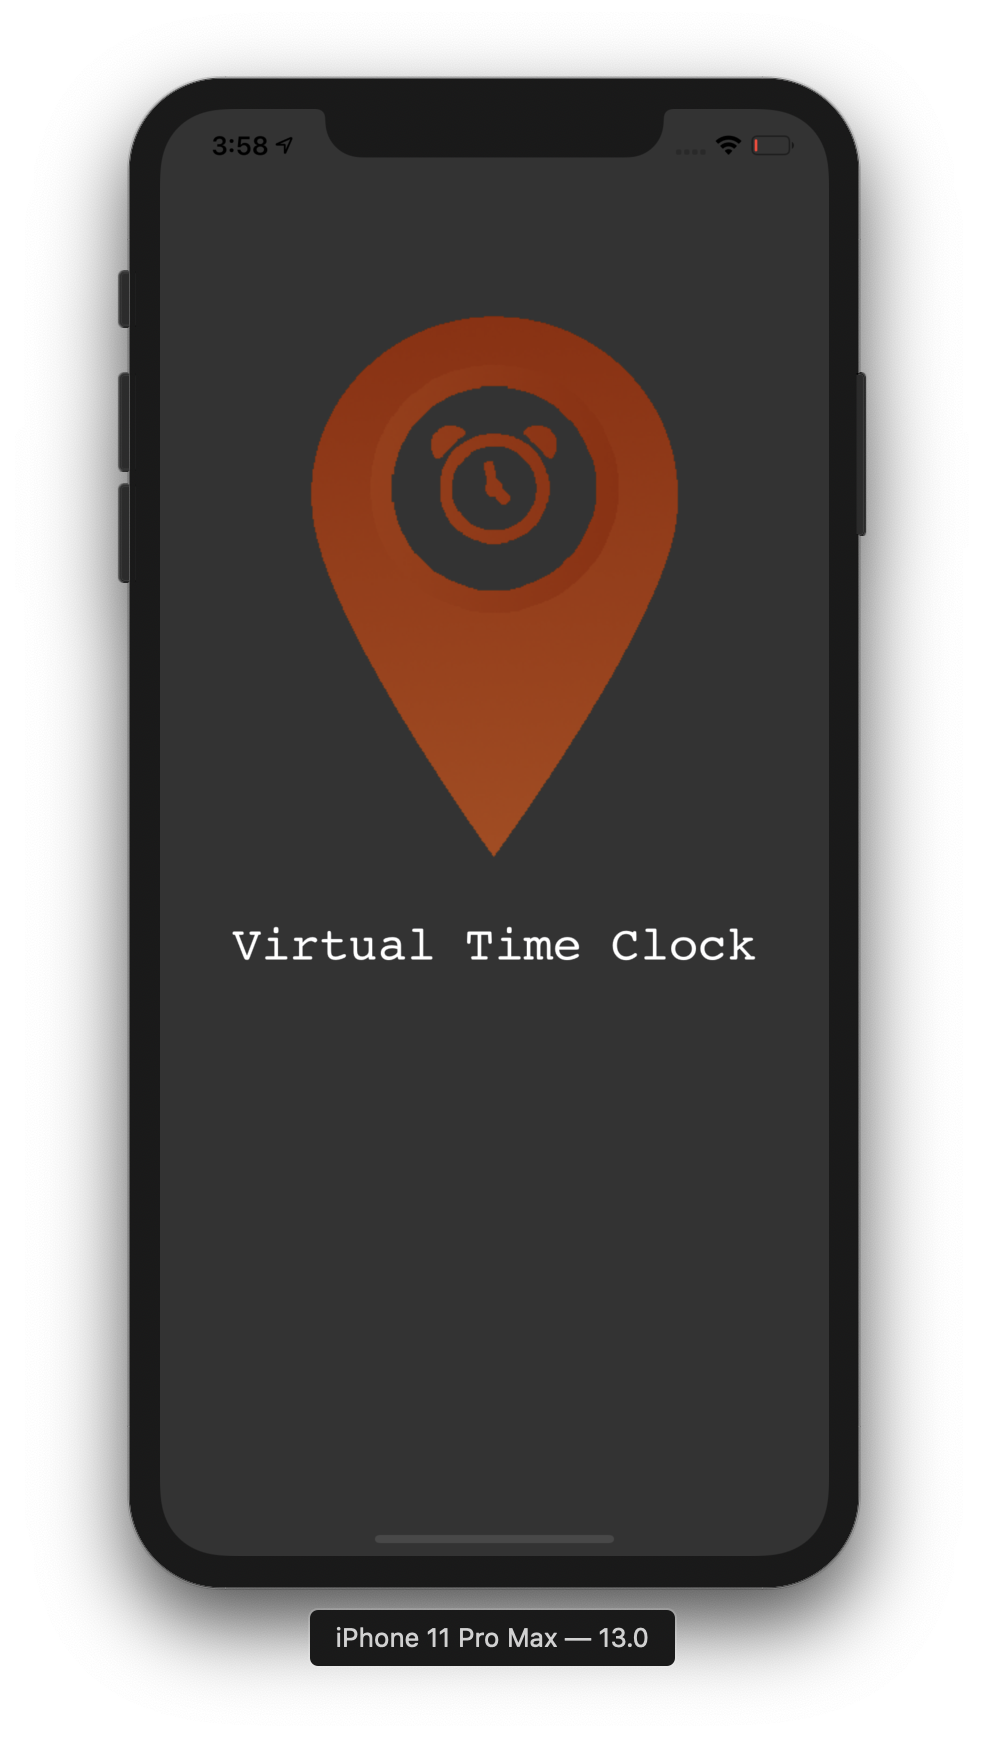
\includegraphics[scale=0.2]{splashScreenIOS.png}
\end{center}

\newpage

\section{Application des employés}

Pour un employé, l'application permet de consulter les différentes missions de l'entreprise et de les consulter. Celui-ci peut ensuite indiquer qu'il est sur les lieux de la mission, ce qui va enclencher un suivi automatique de ses entrées et sorties dans la zone de la mission. De plus, il pourra faire un rapport de l'avancé des travaux pour la ou les mission(s) qu'il a traité durant la journée.

\subsection{Architecture de l'application}

\begin{center}
  \centerline{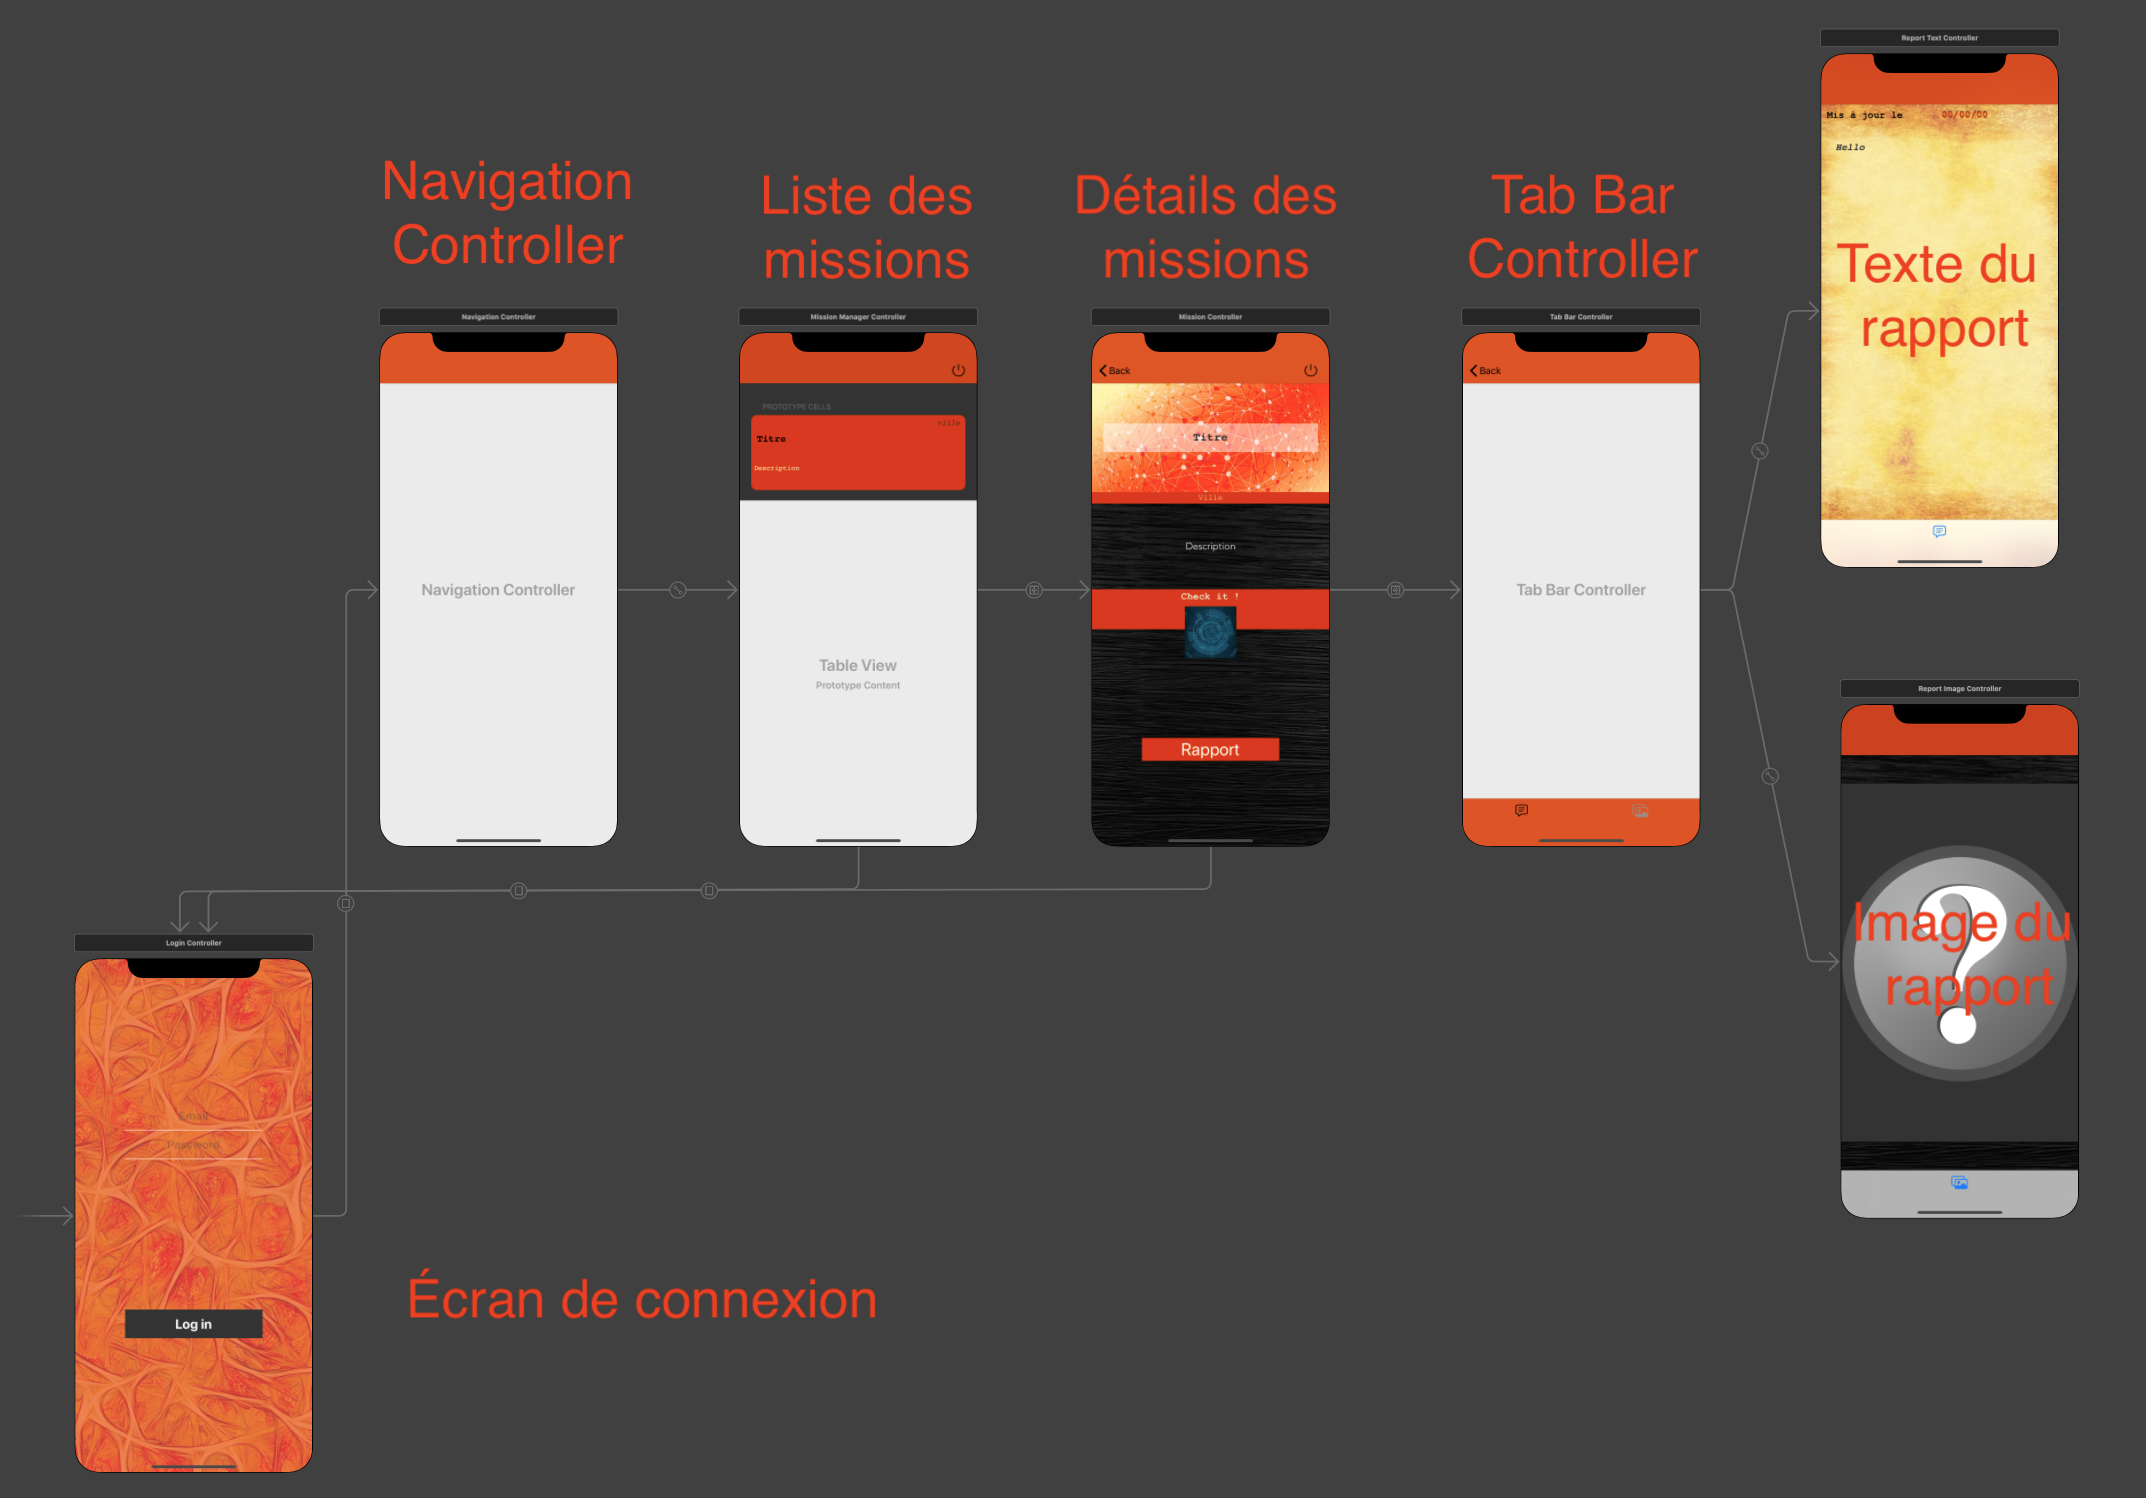
\includegraphics[scale=0.4]{archiIOS.png}}
\end{center}

\newpage

\subsection{Connexion d'un employé}

\begin{center}
  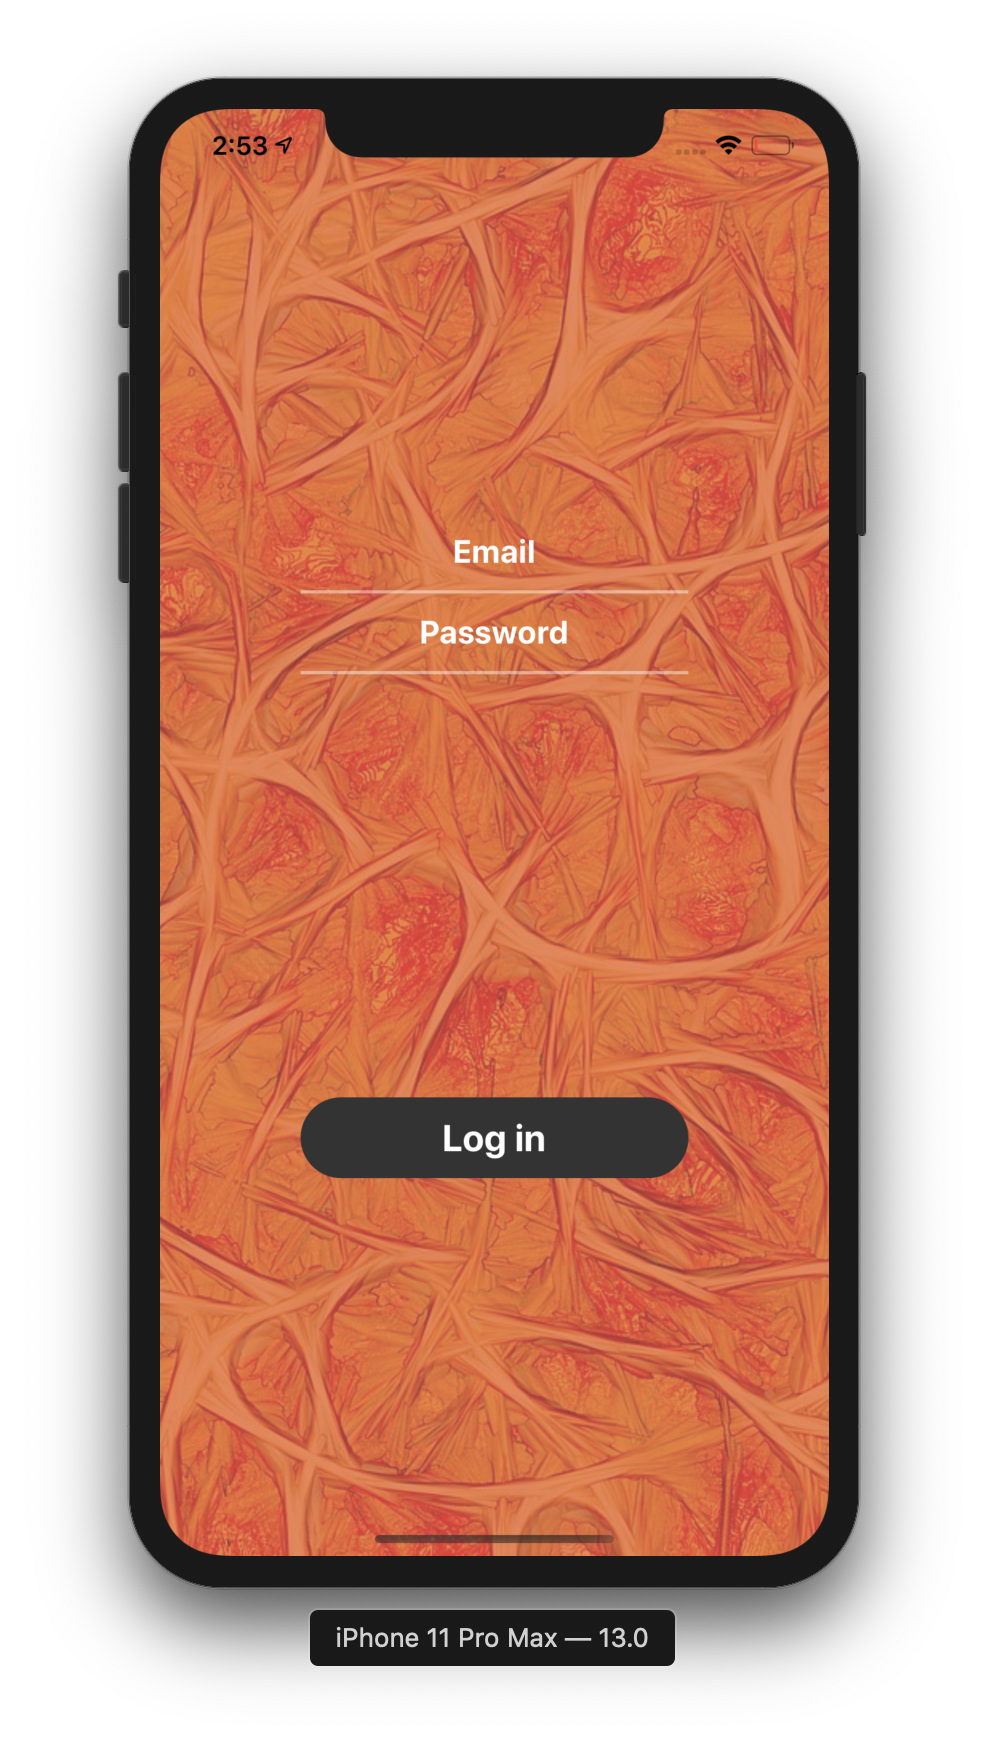
\includegraphics[scale=0.2]{loginIOS.png}
  
\includegraphics[scale=0.15]{loginAnd.jpg}
\end{center}


Pour se connecter, un employé a besoin de son adresse email et de son mot de passe. Ces identifiants sont créés et fournis par le gérant de l'entreprise à chacun de ses employés. Si les identifiants rentrés sont ceux d'un gérant, alors la connexion échoue. De plus, une fois connecté, l'employé reste connecté jusqu'à ce qu'il se déconnecte, même si il quitte l'application. Si il est déjà connecté, il sera directement redirigé vers la liste des missions grâce à cette portion de code :

Dans ViewDidLoad : 
\begin{verbatim}
    // On va tester si un utilisateur est déjà connecté. Si c'est le cas, 
    // on le redirige vers la liste des missions.
        if let user = Auth.auth().currentUser {
            print("un utilisateur est déjà connecté : \(user.email ?? "")")
            perform(#selector(presentMissionManagerController), with: nil, afterDelay: 0)
            // Ici, on utilise un sélector pour s'assurer que la vue vers laquelle
            // on veut rediriger l'utilisateur soit belle et bien chargée.
        } else {
            print("Aucun utilisateur n'est connecté.")
        }
        
// Fonction appelée si un utilisateur est déjà connecté
     @objc private func presentMissionManagerController() {
         self.performSegue(withIdentifier: "loginToMissionManager", sender: self)
     }
\end{verbatim}

De plus, dans cette vue, le clavier peut être fermé en cliquant n'importe où sur l'écran grâce à un \textbf{TapGesture}. 

\newpage

\subsection{Liste des missions}

\begin{center}
  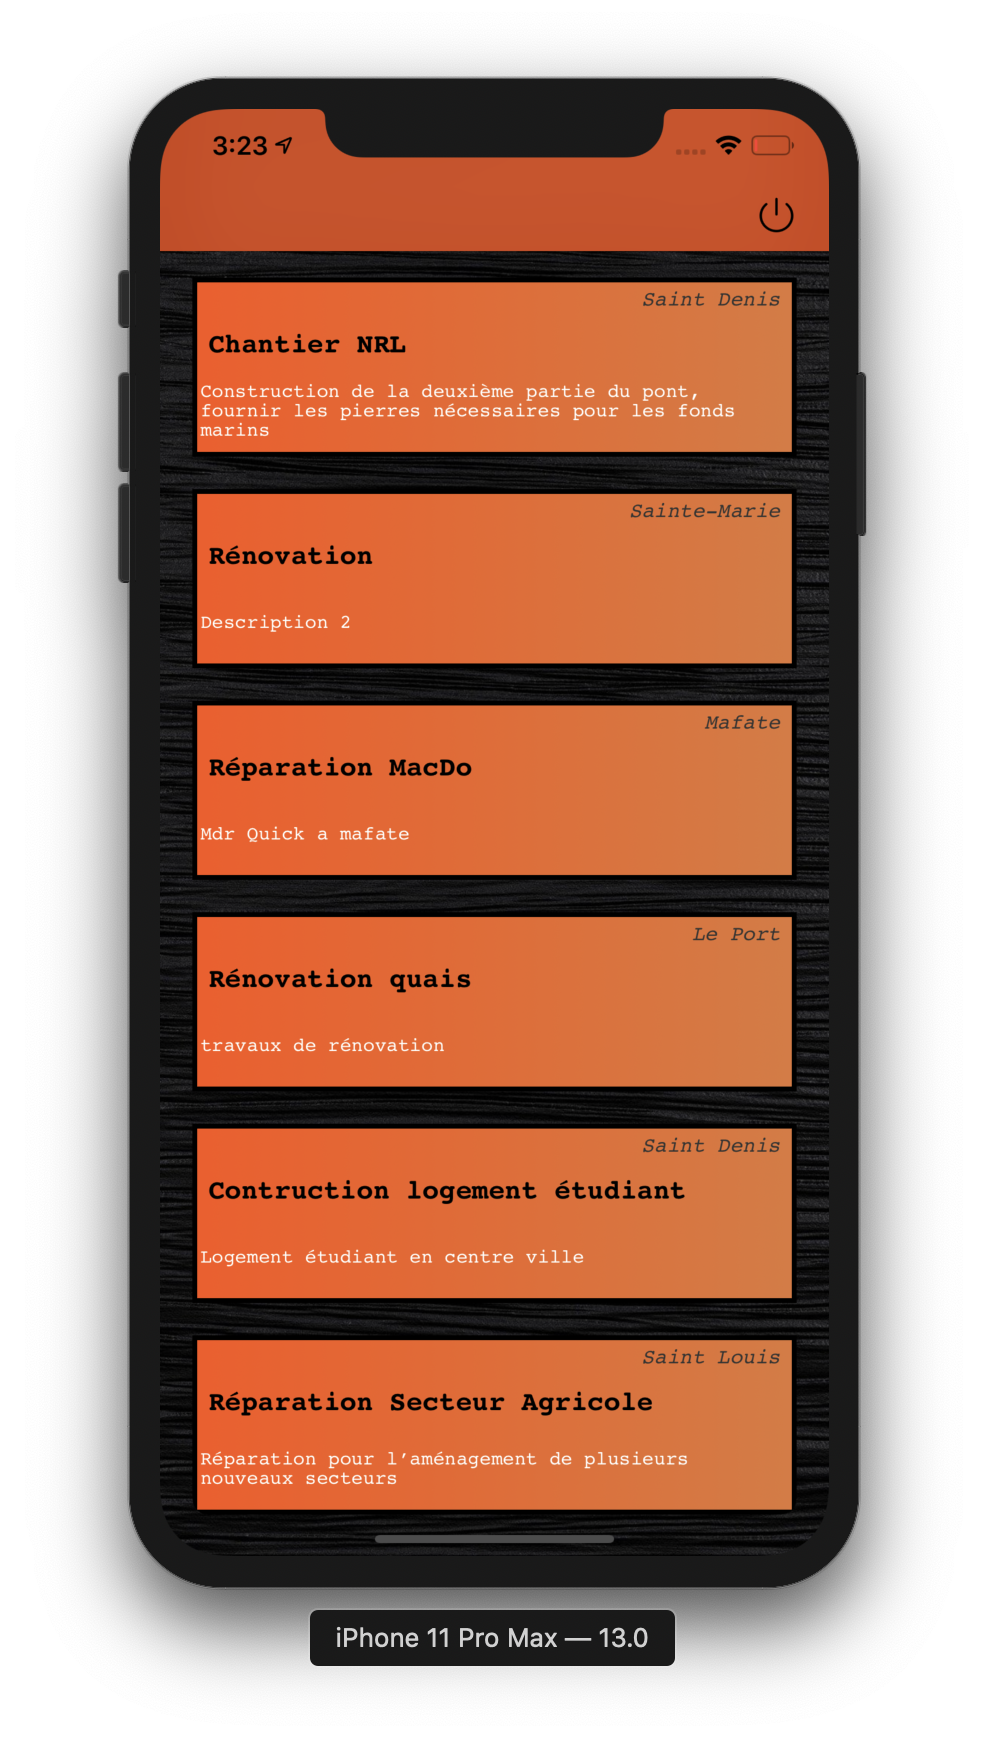
\includegraphics[scale=0.2]{ListeMissionsIOS.png}
  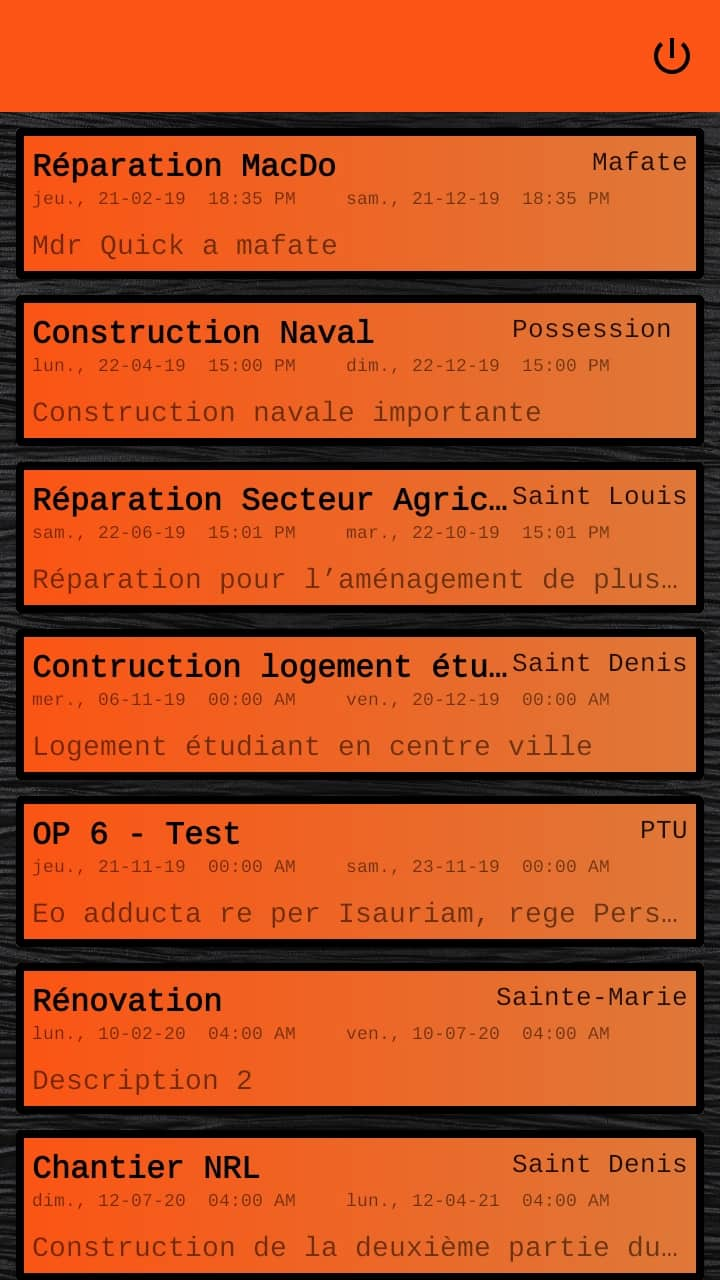
\includegraphics[scale=0.15]{missionsAnd.jpg}
\end{center}

Cet écran permet à l'employé de consulter les différentes missions de l'entreprise et de choisir celle sur laquelle il doit travailler.
C'est ici que chaque mission est chargée dans l'application depuis la base de données. Pour chacune des missions, une instance de la classe \textbf{Mission}  est créée et est stockée dans la liste "\textbf{missions}" avant d'être affichée dans la \textit{TableView}.
Ensuite, lorsque l'employé clique sur une mission, l'instance de la classe \textbf{Mission} correspondante est passée à la vue suivante comme cela : 


\begin{verbatim}
// Fontion permettant de faire des actions avant l'envoi du segue
    override func prepare(for segue: UIStoryboardSegue, sender: Any?) {
        
        // On test si le segue est bien celui qu'on espère
        if segue.identifier == "MissionsManagerToMission" {
            
            // Récupération de la destination du segue
            let destination = segue.destination as! MissionController
            
            let mission = sender as! Mission
            destination.mission = mission
        }
     }
\end{verbatim}

\newpage

\subsection{Détails d'une mission}

\begin{center}
  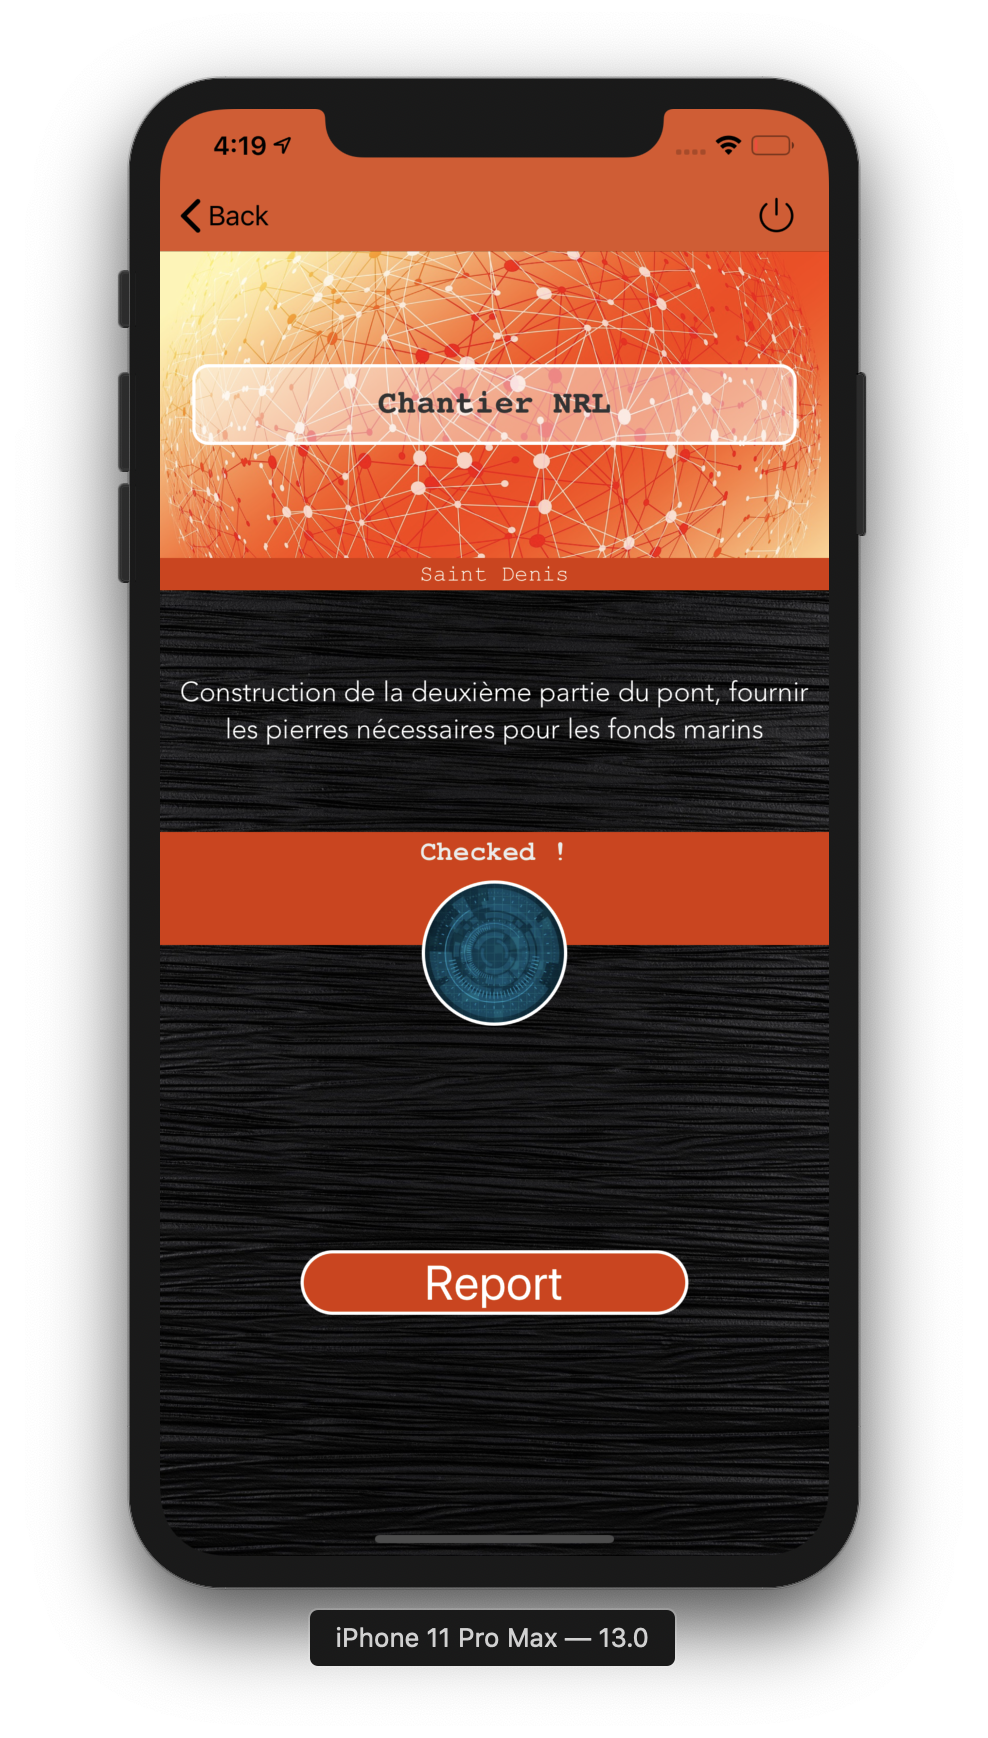
\includegraphics[scale=0.2]{DetailMissionIOS.png}
  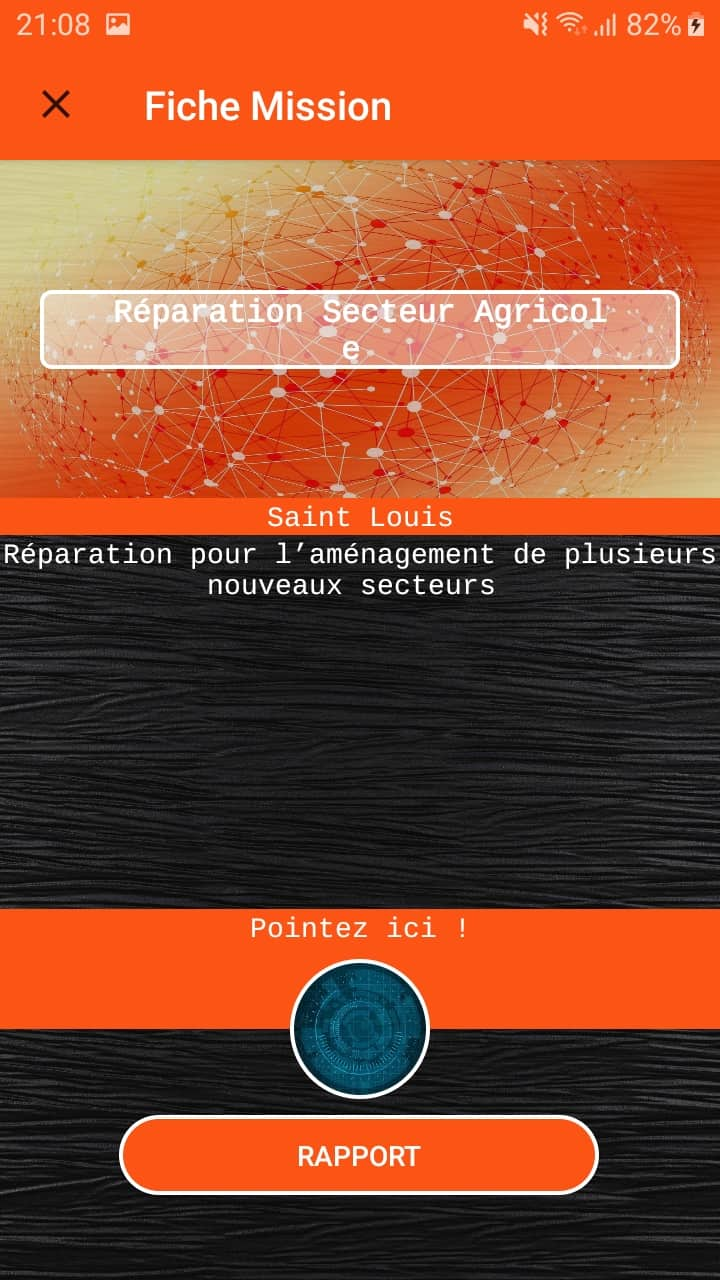
\includegraphics[scale=0.15]{missionAnd.jpg}
\end{center}

Lorsq'un employé clique sur une mission, le détail de celle-ci s'affiche. Cette vue permet également à l'employer de pointer et de se diriger vers les écrans dédiés au rapport de cette mission.
C'est également dans cette vue que le rapport de la mission est récupéré depuis la base de données, si il existe, puis celui-ci est transformé en une instance de la classe \textbf{Rapport}. 
Voici le code de récupération du rapport stocké dans la base de données :
\begin{verbatim}
// Fonction permettant de récupérer le rapport de la mission courante dans la BD
    private func getReportFromDB(forMissionId: String) {
        if missionID != "" {
            let missionsRef = database.collection("missions").document(missionID)
            
            missionsRef.getDocument { (document, error) in
                // On test si le document lié à cette mission existe bien
                if let document = document, document.exists {
                    // On récupère le rapport stocké dans le document. C'est un dictionnaire.
                    let rapportFromDB: [String: Any]? = document.get("rapport") as? [String: Any]
                    
                    if rapportFromDB != nil { // Si un rapport existe sur la base de données,
                        // On va récupérer les données de ce rapport :           
                        let texte: String = rapportFromDB!["texte"] as! String  
                        // ... Récupération des autres inforamtions ...
                        // On récupère ce rapport sous forme d'objet 
                        self.rapport =  Rapport(texte: texte, imagePath: imagePath, date: date)
                    } else { print("Il n'existe pas de rapport pour cette mission.") }
                } else {
                    print("Erreur : Le document demandé pour cette mission n'existe pas !")
                    self.view.makeToast(NSLocalizedString("missionNotExist",
                    comment: "Alert message"), duration: 1.5) }}} }
\end{verbatim}

\subsection{Pointage et contrôle d'assiduité automatique}

Cette partie est la fonctionnalité principale de l'application, et permet au gérant de savoir si un employé se trouve sur les lieux de la mission à n'importe quel moment.
Lorsqu'un employé clique sur le bouton de pointage le processus suivant s'enclenche et continue même si l'application fonctionne en \textbf{arrière plan} :

\newpage

\begin{center}
  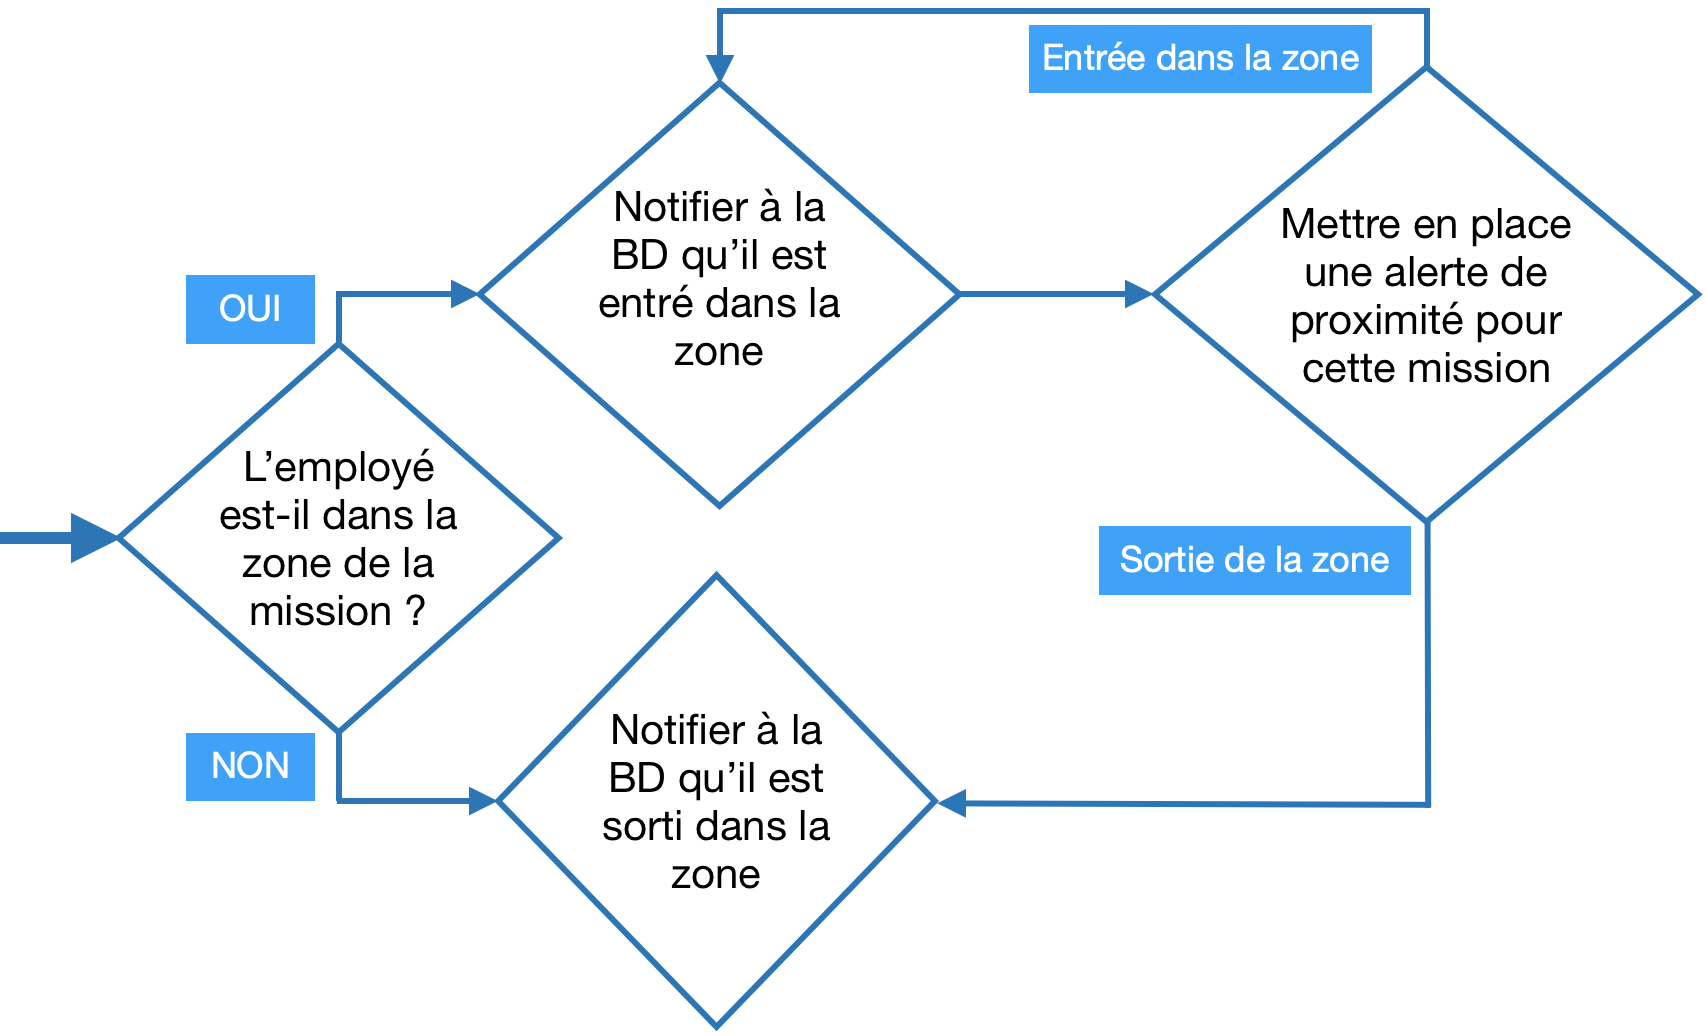
\includegraphics[scale=0.4]{geolocalisationProcess.png}
\end{center}

Dans la version iOS, toute la partie gestion des alerte de proximité est faite par la classe \textbf{LocationAreaManager} qui est un \textit{Singleton Design Pattern} \cite{Singleton}. Le singleton nous permet de nous assurer que cette classe n'est instanciée qu'une seule et unique fois dans le code, grâce notamment à une constante \textit{static} contenant l'instance de la classe au sein même de la classe.

\begin{verbatim}
class LocationAreaManager{
    
    static let shared = LocationAreaManager()
    
    let manager = CLLocationManager()
    let database = Firestore.firestore()
    var locationGranted: Bool?
    var currentArea: CLCircularRegion?
    
    private init(){ }
    ...
\end{verbatim}


Grâce à \textbf{LocationAreaManager}, il est maintenant possible de stocker les différentes zones d'alerte de proximité activées, ce qui nous a permis de faire en sorte d'avoir toujours une seule et unique zone en monitoring (Car nous considérons que l'employé ne travail que sur une seule mission à la fois). Cela est géré par la fonction suivante, de la classe \textbf{LocationAreaManager} :

\begin{verbatim}
func startMonitoringForNewArea(newArea:CLCircularRegion, userID:String, mission: Mission){
        if currentArea != nil {
            manager.stopMonitoring(for: currentArea!)
            notifyExitToDB(userID: userID, mission: mission)
        }
        manager.startMonitoring(for: newArea)
        currentArea = newArea
    }
\end{verbatim}

\newpage


\subsection{Rapport de mission}

\subsubsection{Texte du rapport}

\begin{center}
  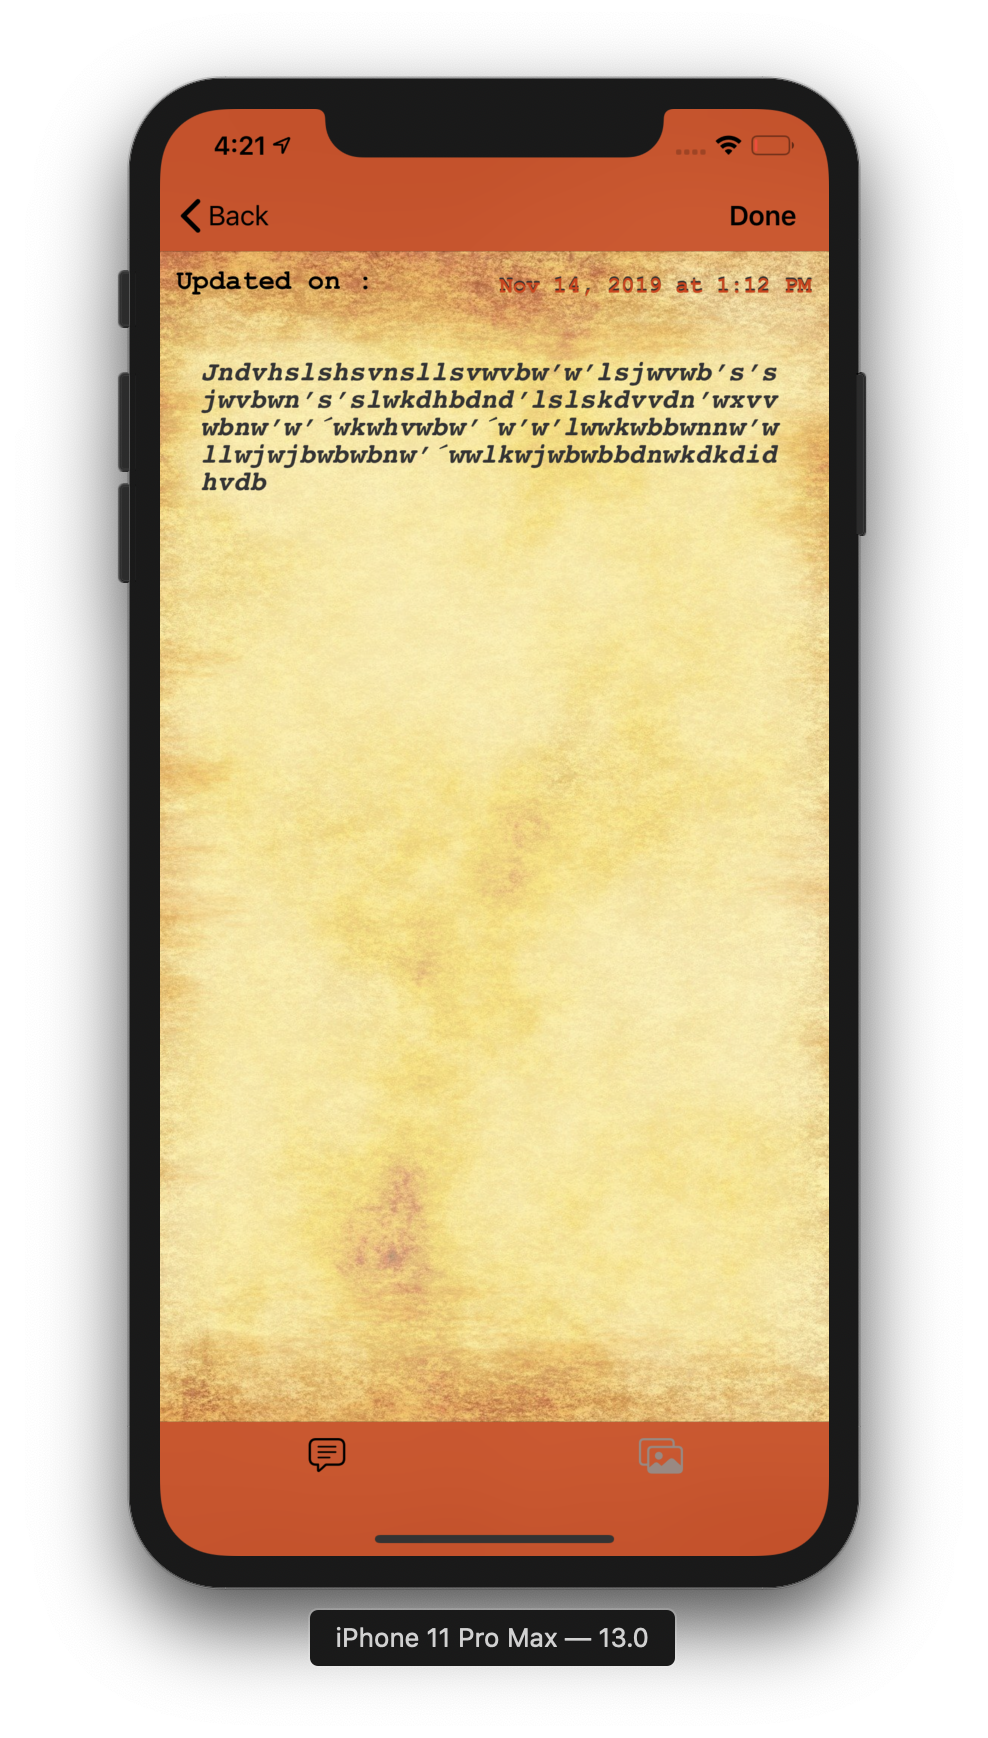
\includegraphics[scale=0.2]{TextRapportIOS.png}
  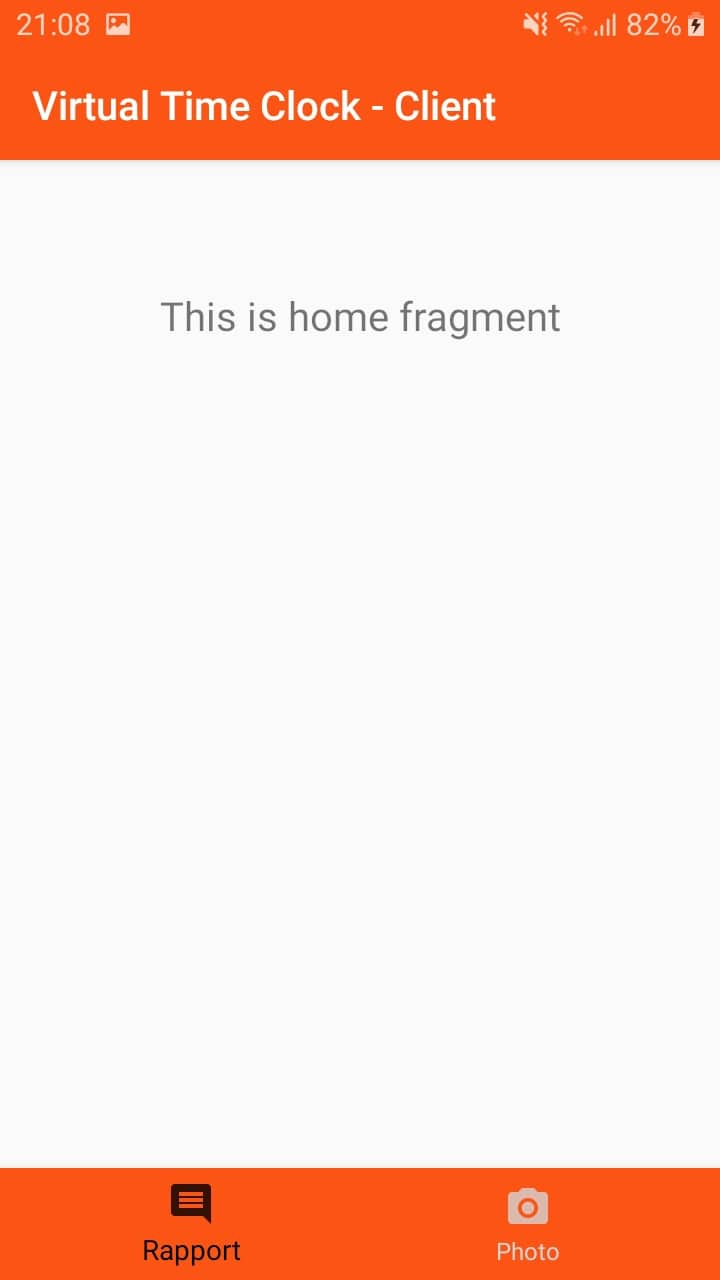
\includegraphics[scale=0.15]{texteAnd.jpg}
\end{center}

Dans cette vue, l'employé peut consulter et modifier le texte du rapport de la mission courrante. En secouant le téléphone pendant plus de 0.5 secondes, il peut supprimer tout le texte d'un coup.
Voici le code (condensé) de l'utilisation de l'accéléromètre : 

\begin{verbatim}
private func listenDeviceMovement(){
    // On va utiliser les données pré-traitées de l'accéléromètre
    if motionManager.isDeviceMotionAvailable {
        motionManager.deviceMotionUpdateInterval = 0.1 // Interval de prélèvement des valeurs
        motionManager.startDeviceMotionUpdates(to: .main) { (dm, error) in
            let accelerationX = dm?.userAcceleration.x  // Accélération sur l'axe X
            let accelerationY = dm?.userAcceleration.y  // Accélération sur l'axe Y
            let accelerationZ = dm?.userAcceleration.z  // Accélération sur l'axe Z
            let now = Date() // Date actuelle

        // Si on détecte une secousse
        if abs(accelerationX!) > 0.5 || abs(accelerationY!) > 0.5 || abs(accelerationZ!) > 0.5 {
          if !self.isMovingPhone { // Si le téléphone n'est pas en état "moving"
          	self.lastTimeCheck = now    // On lance le chrono, en sauvegardant l'heure actuelle
          	self.isMovingPhone = true   // Le téléphone est dans l'état "moving"
          } else if now.timeIntervalSince(self.lastTimeCheck!) >= 0.5 { //Secousse >0.5 secondes
          	self.reportTextView.text = ""   // On efface le texte
          	self.isMovingPhone = false      // Le téléphone n'est plus dans l'état "moving"
        }
        } else {
        // Le téléphone ne bouge plus, il n'est plus dans l'état "moving"
        self.isMovingPhone = false
        }
    } } }
\end{verbatim}

\newpage

\subsubsection{Image du rapport}

\begin{center}
	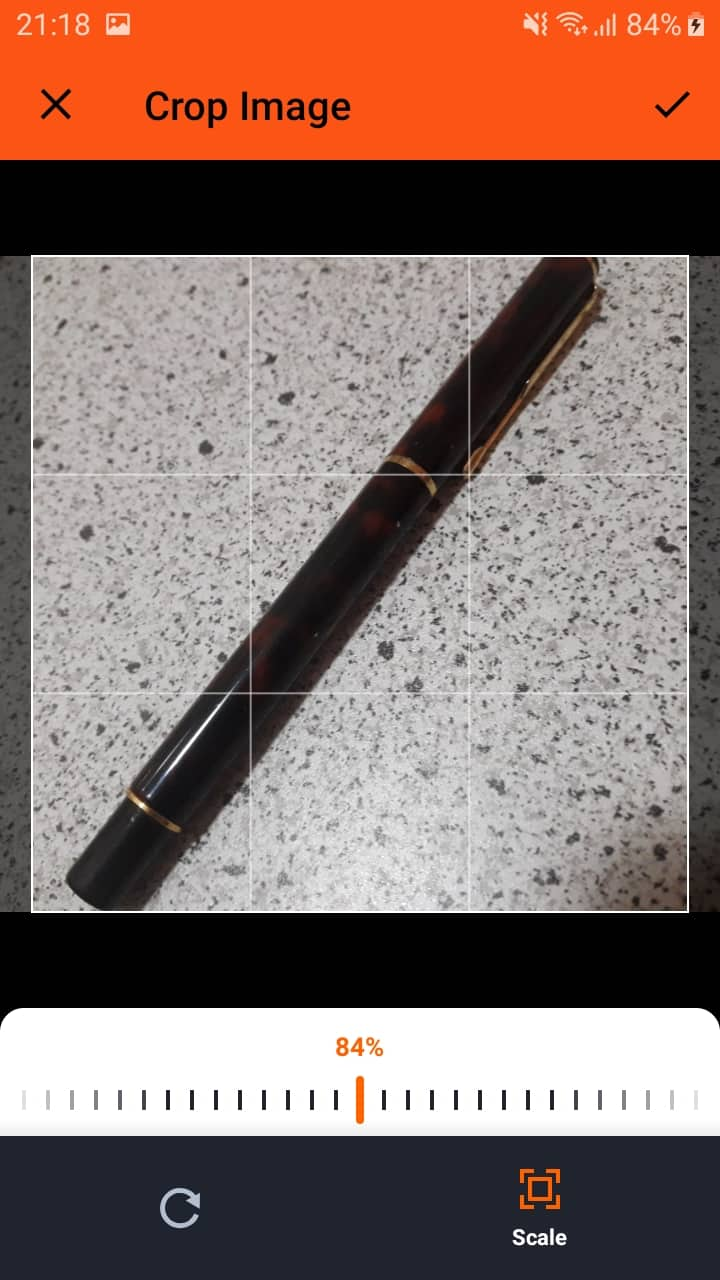
\includegraphics[scale=0.15]{photoAnd.jpg}
  	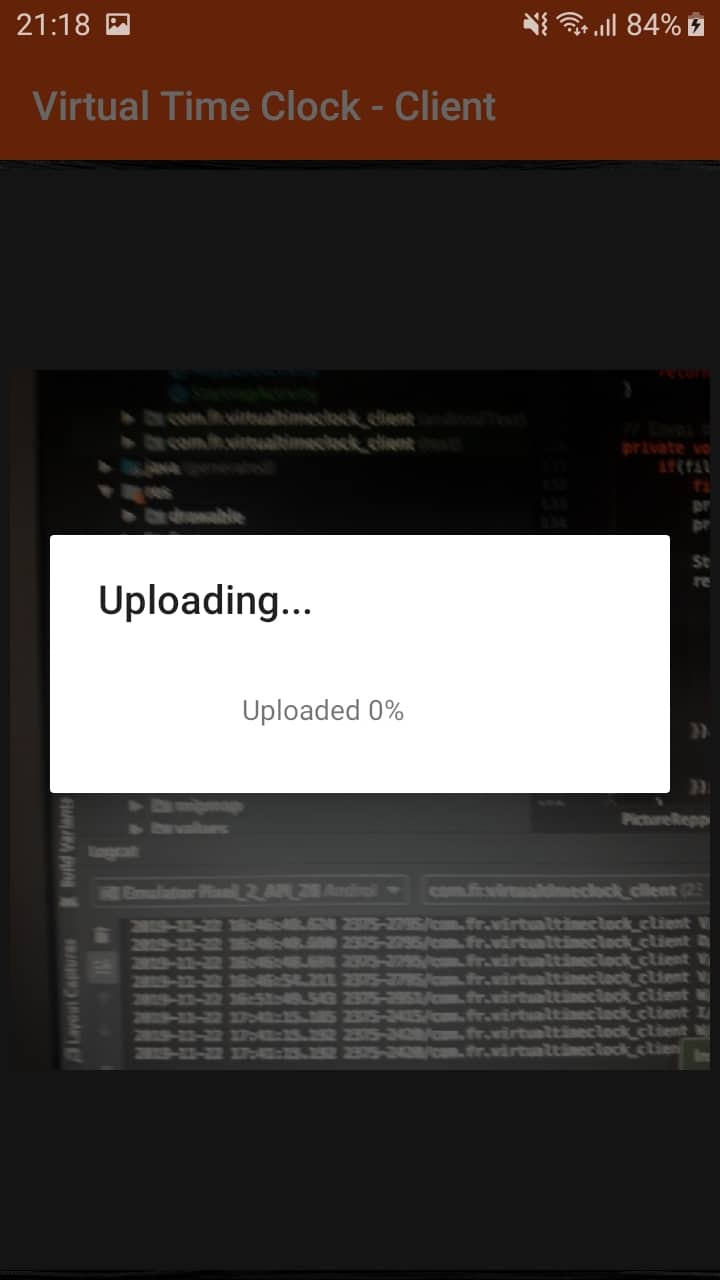
\includegraphics[scale=0.15]{photoUpdateAnd.jpg}
  	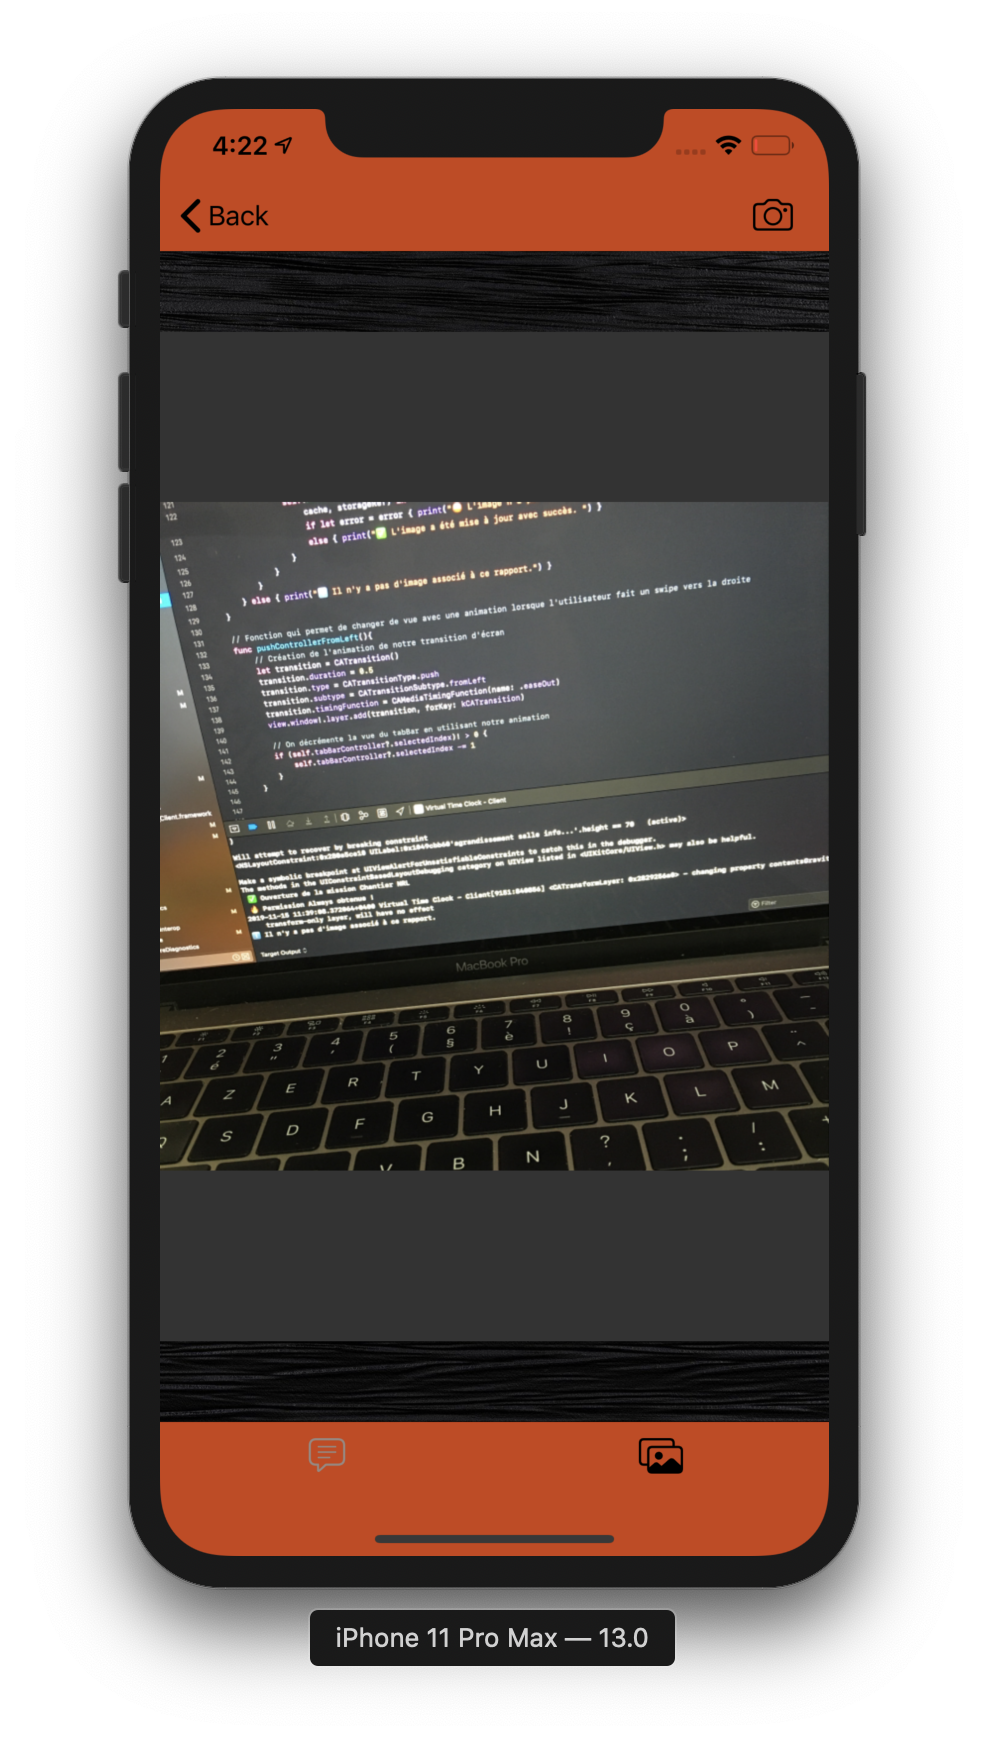
\includegraphics[scale=0.2]{ImageRapportIOS.png}
\end{center}
 
 En complément du texte, l'employé peut consulter/ajouter une image au rapport. Pour celà, il utilise l'appareil photo du téléphone. Voici le code permettant d'ouvrir la l'appareil photo :
 \begin{verbatim}
 @objc func openCamera(){
       // On vérifie si le téléphone a un appareil photo
       if UIImagePickerController.isSourceTypeAvailable(UIImagePickerController.SourceType.camera) { 
           let imagePicker = UIImagePickerController() //Utilisation de l'appareil photo iOS
           imagePicker.delegate = self
           imagePicker.sourceType = .camera //Utilisation de la caméra uniquement
           imagePicker.allowsEditing = true //On autorise l'édition de l'image
           self.present(imagePicker, animated: true, completion: nil) //On affiche la vue
       } }
 \end{verbatim}
 
 
 \subsubsection{Navigation dans le TabBar grâce aux geste courrants}
Pour naviguer entre le texte et l'image de rapport, l'employé peut "swiper".
Lorsque le \textit{SwipeGesture} est détecté de la manière suivante ...

\begin{verbatim}
let swipeLeft = UISwipeGestureRecognizer(target: self, action: #selector(onSwipeGesture))
swipeLeft.direction = .left
self.view.addGestureRecognizer(swipeLeft)
\end{verbatim}

... l'écran est "poussé" grâce à une transition. Voici le code : 

\begin{verbatim}
func pushControllerFromRight(){
        let transition = CATransition() //Création de l'animation de transition d'écran
        transition.duration = 0.5
        transition.type = CATransitionType.push
        transition.subtype = CATransitionSubtype.fromRight
        transition.timingFunction = CAMediaTimingFunction(name: .easeOut)
        view.window!.layer.add(transition, forKey: kCATransition)
        // On incrémente la vue du tabBar en utilisant notre animation
        if (self.tabBarController?.selectedIndex)! < 2 {
            self.tabBarController?.selectedIndex += 1
        }}
\end{verbatim}

\newpage

\subsection{Déconnexion}

L'utilisateur peut se déconnecter grâce au bouton se trouvant dans la barre de navigation. Si il se déconnecte, il sera redirigé vers l'écran de connexion et devra s'authentifier pour accéder à l'application.
\begin{center}
  
\includegraphics[scale=0.5]{logoutIOS.png}
\end{center}

La déconnexion de l'utilisateur se fait grâce à Firebase, via le code suivant en java  : \begin{verbatim}
 private void userLogout() {
        mAuth.getInstance().signOut();
        Intent intent = new Intent(MissionManagerActivity.this, LoginActivity.class);
        intent.addFlags(Intent.FLAG_ACTIVITY_CLEAR_TOP);
        intent.addFlags(Intent.FLAG_ACTIVITY_CLEAR_TASK);
        startActivity(intent);
    }
userLogout();
\end{verbatim}



\section{Application des gérants}

Pour un gérant de l'entreprise, l'application lui permettra de gérer ses employés et ses différentes missions. En effet, il pourra consulter la liste des missions et l'avancement de celle-ci grâce au rapport rédigé par les employés mais aussi ajouter de nouvelles missions ou les supprimer. Il pourra également consulter la liste de ses employés, en ajouter de nouveaux.

\subsection{Architecture de l'application}

\begin{center}
    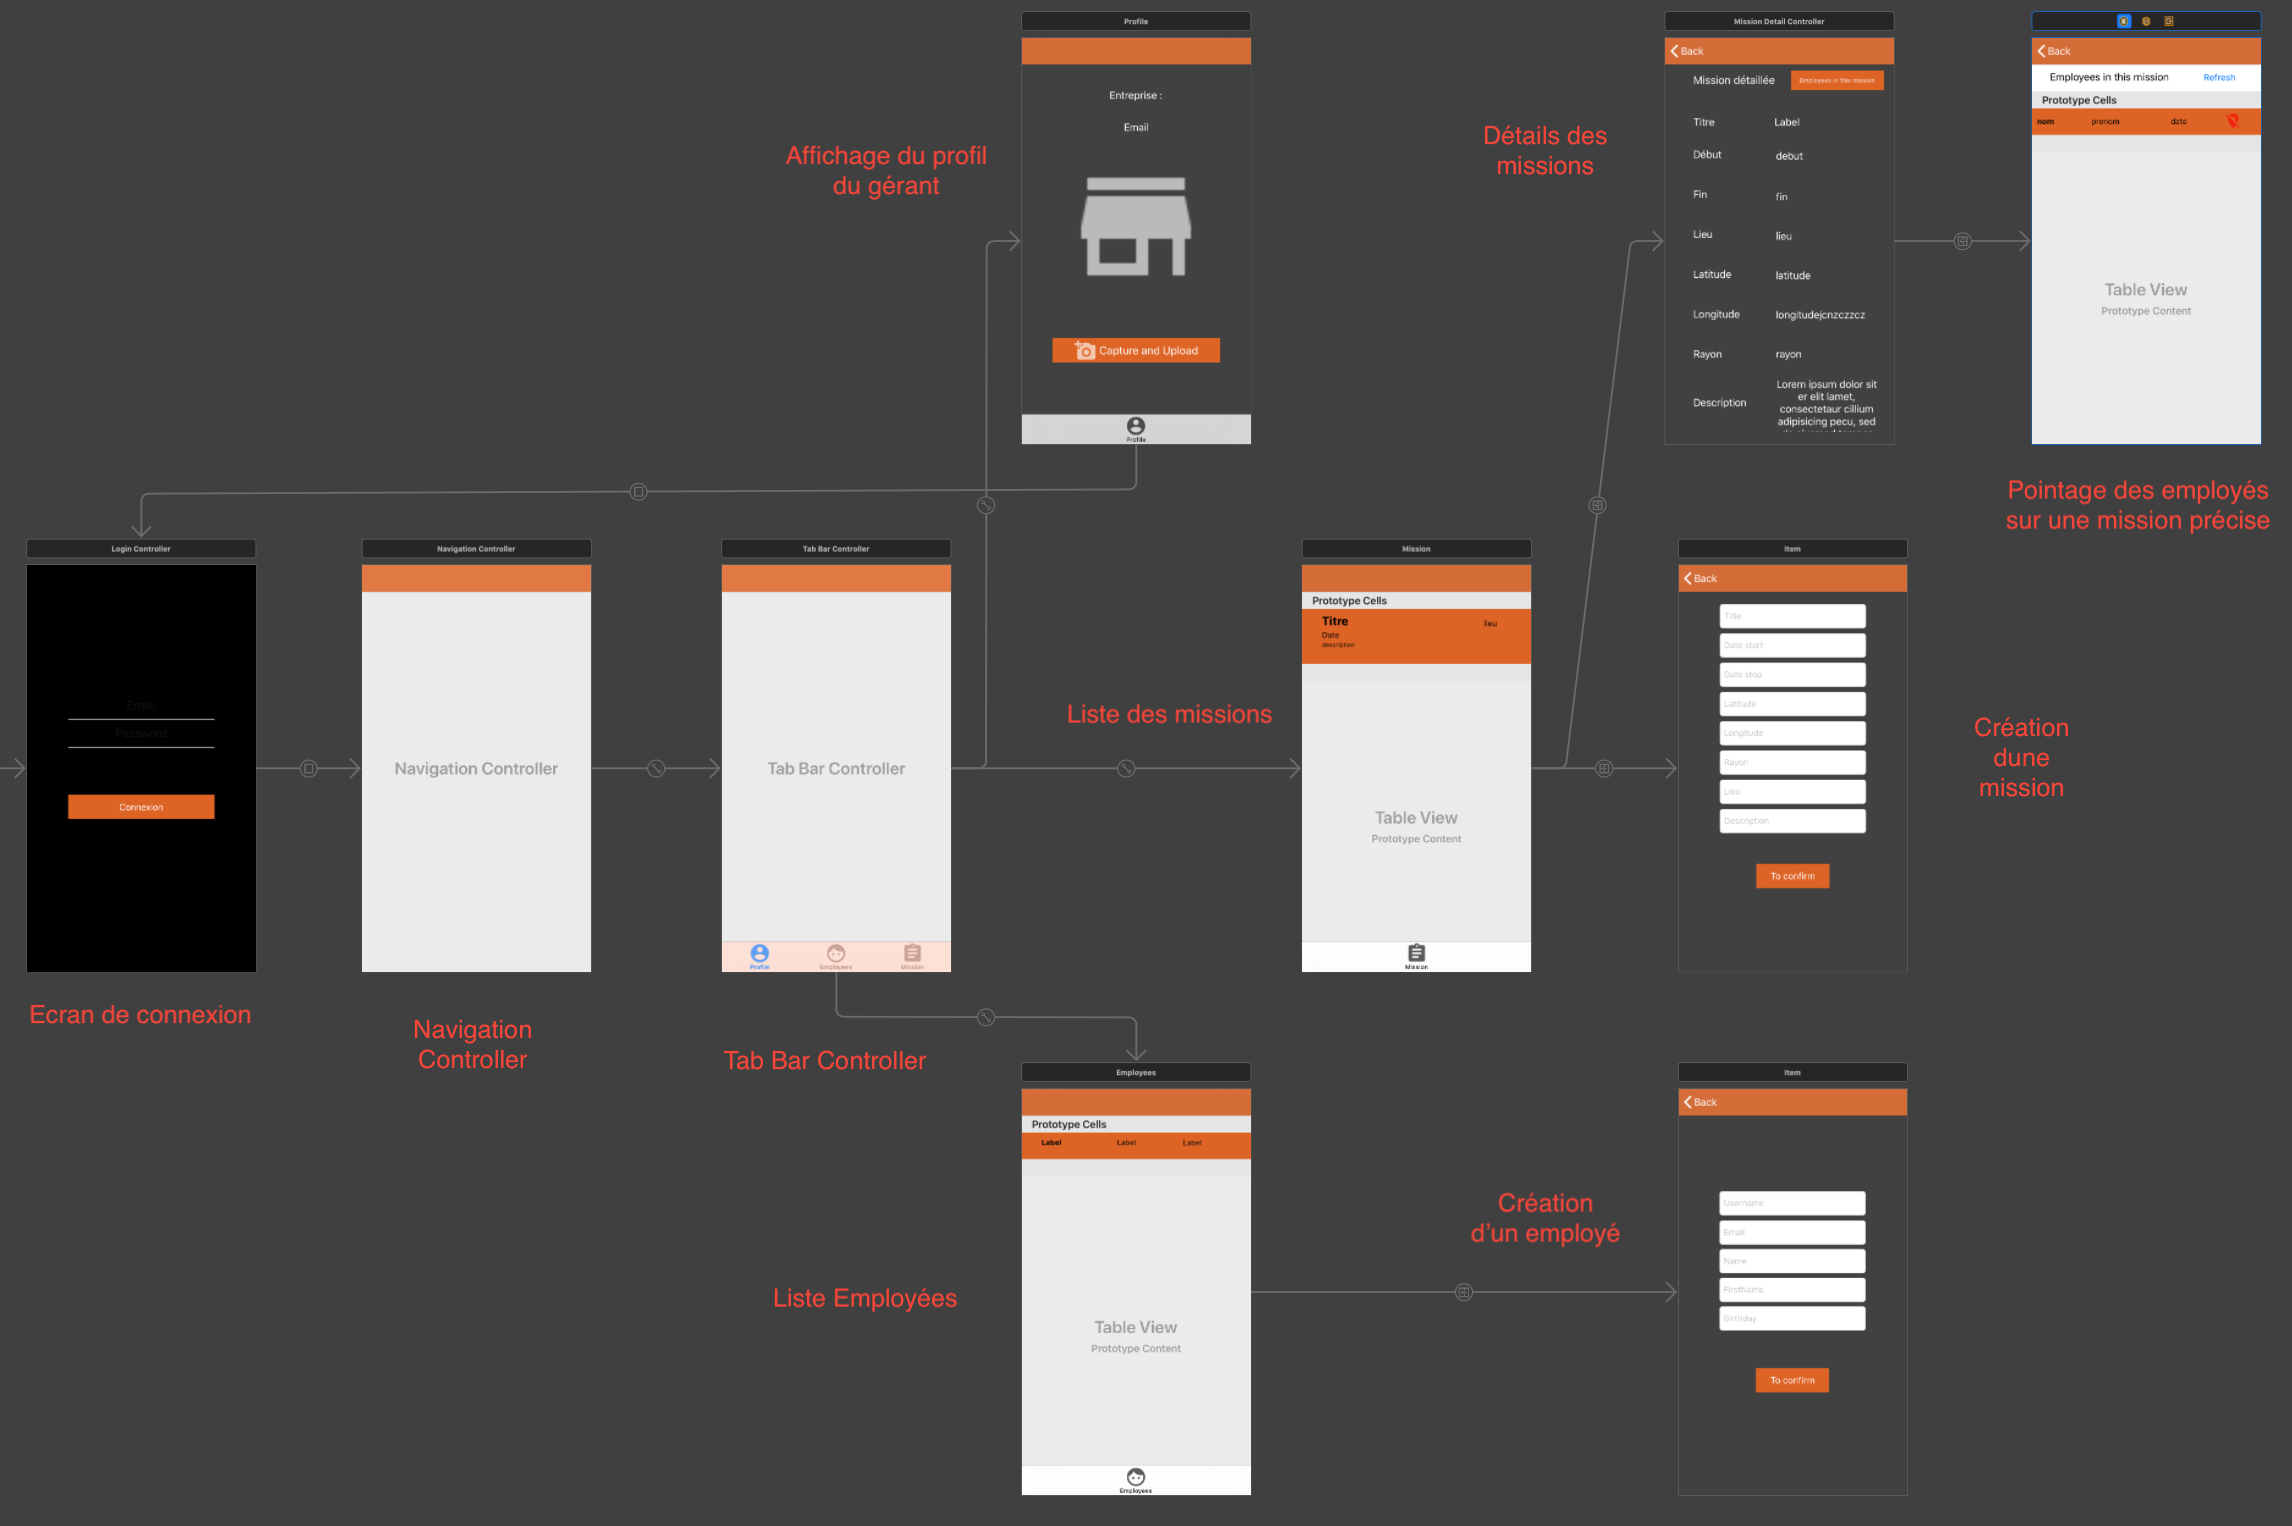
\includegraphics[scale=0.2]{archiGerant.png}
\end{center}

\newpage

\subsection{Connexion du gérant}

\begin{center}
    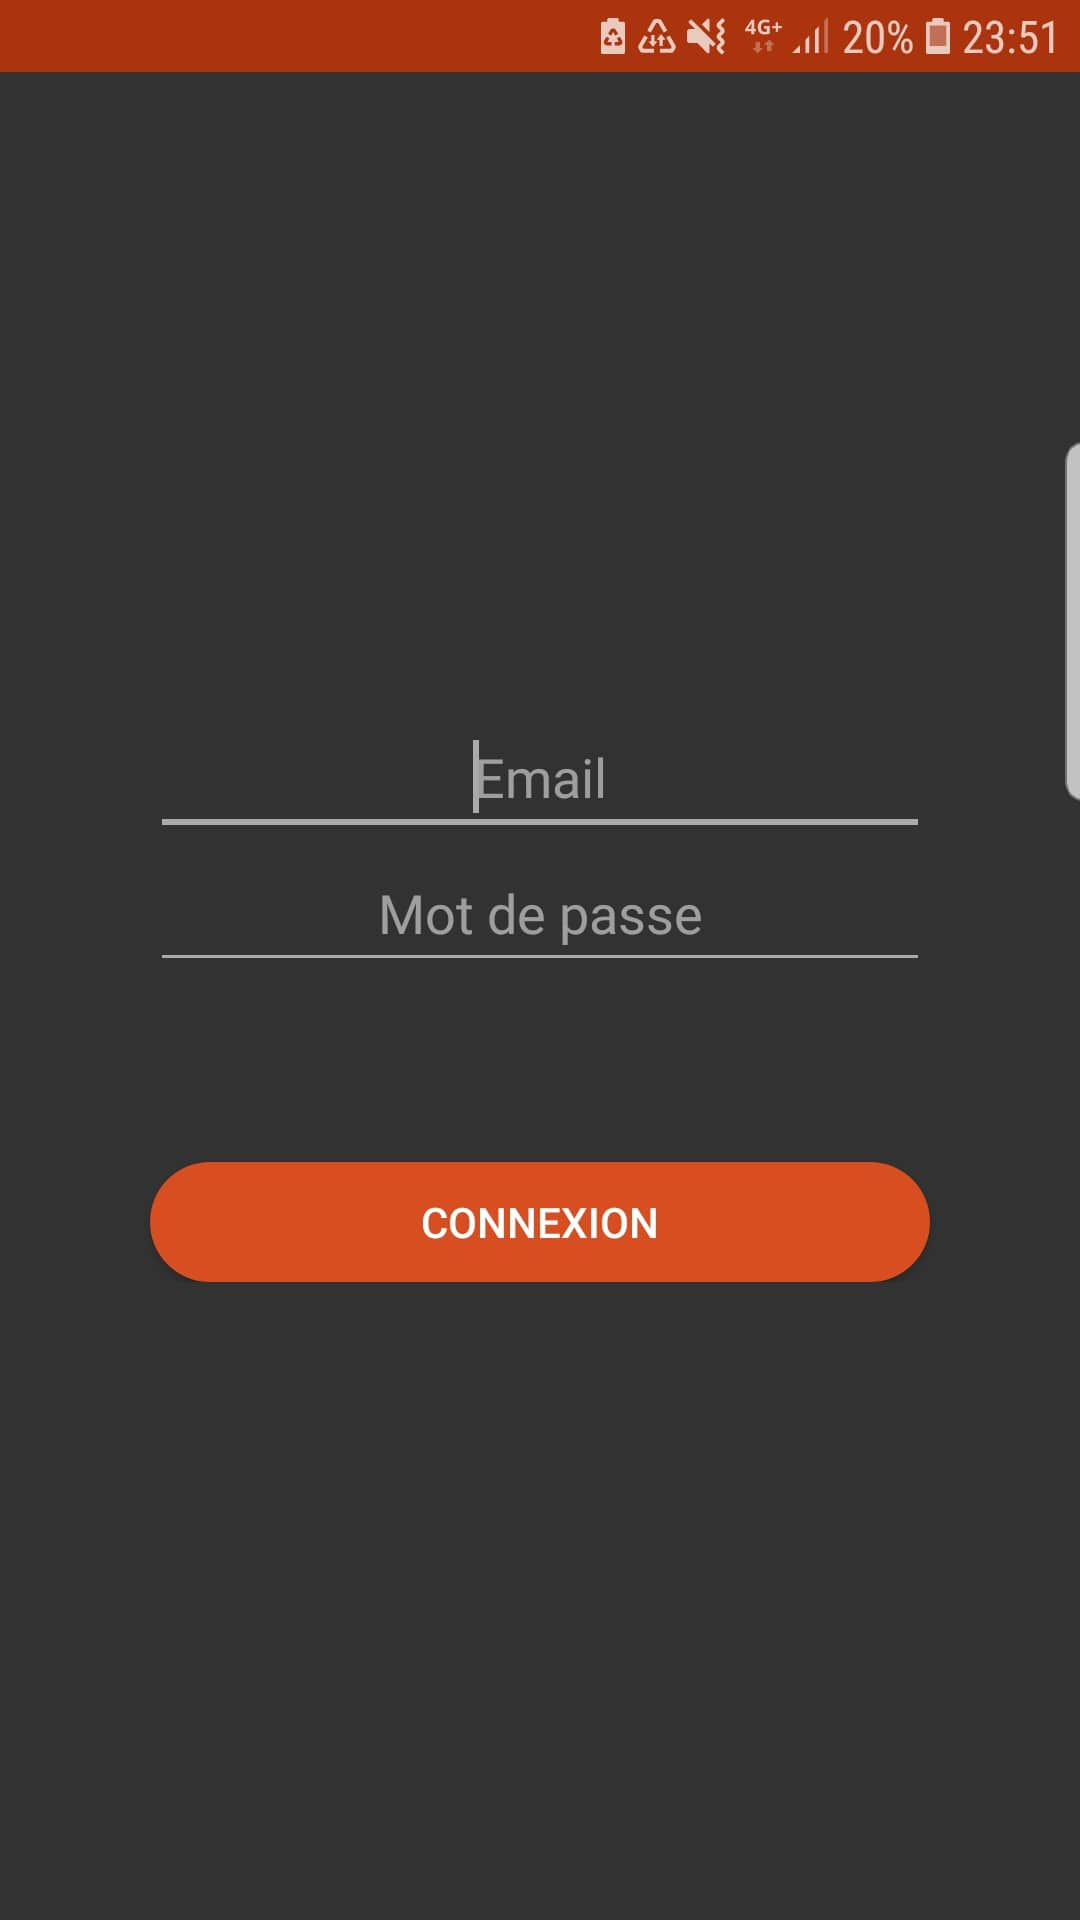
\includegraphics[scale=0.1]{co.jpg}
    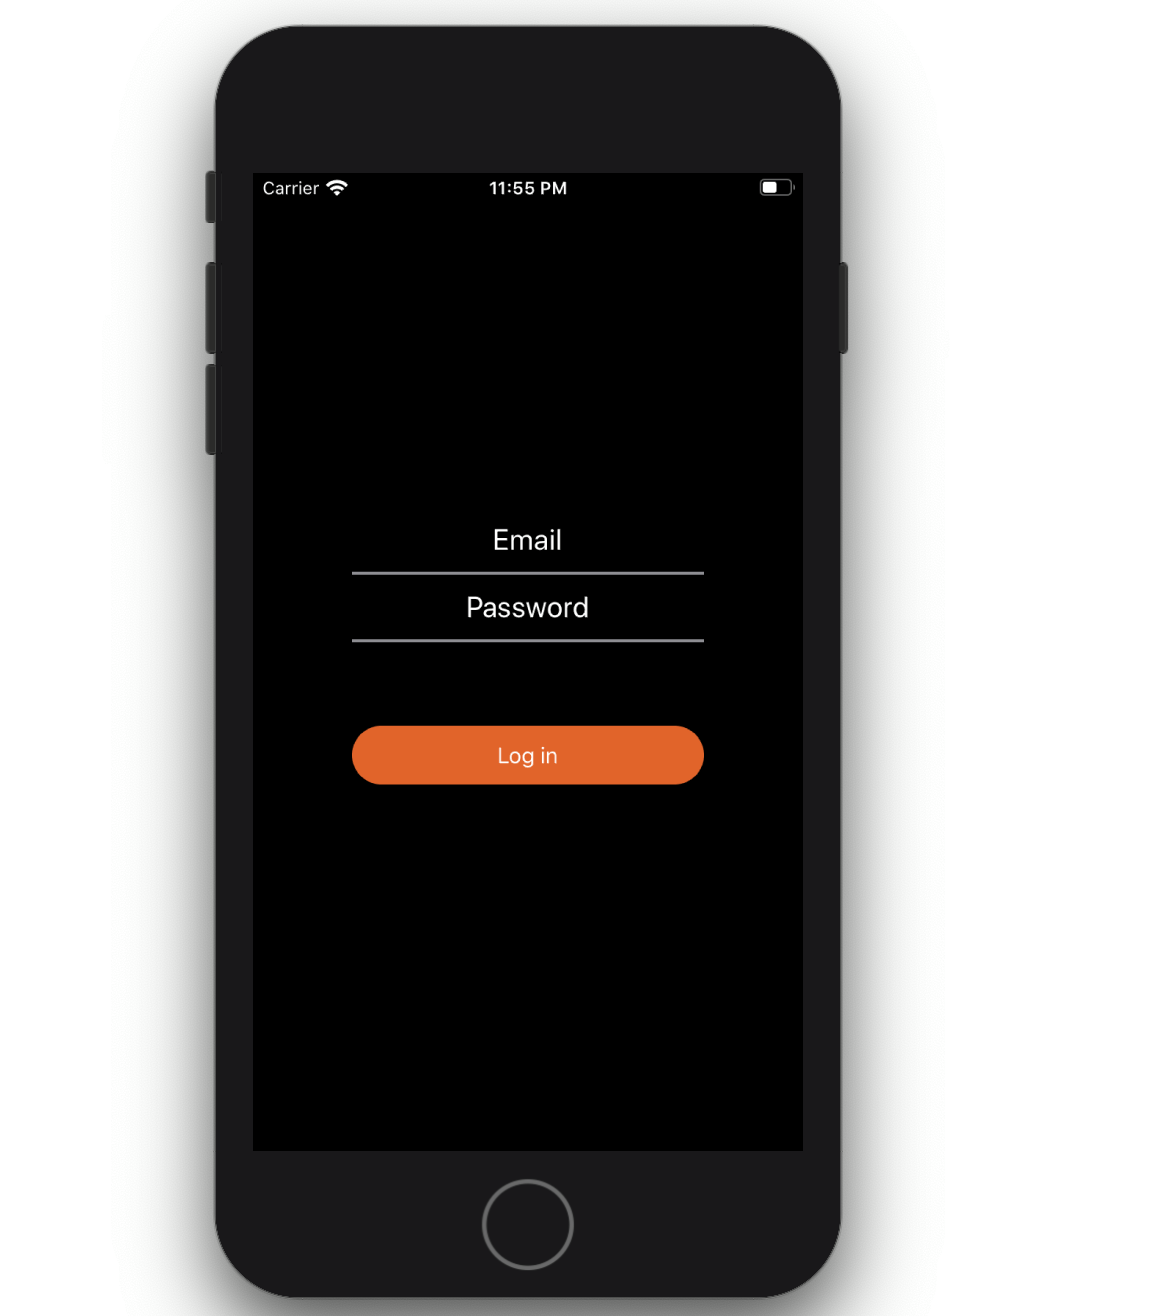
\includegraphics[scale=0.15]{coIOS.png}
\end{center}

Tout comme les employés, les gérants doivent se connecter avec un email et un mot de passe et la connexion se fera seulement si les identifiants sont bien ceux d'un compte gérant. La connexion est aussi maintenue tant qu'il ne se  déconnecte pas et une fois connecté, ils sera redirigé sur le menu principal de l'application grâce à ce code swift :

\begin{verbatim}
    override func viewDidLoad() {
        super.viewDidLoad()
        
        // On va tester si un gérant est déjà connecté. 
        //Si c'est le cas, on le redirige vers son profil
        if let user = Auth.auth().currentUser {
            print("Un gérant est déjà connecté : \(user.email ?? "")")
            perform(#selector(loginagain), with: nil, afterDelay: 0)
            // Ici, on utilise un sélector pour s'assurer que la vue vers laquelle
            // on veut rediriger le  gérant soit belle et bien chargée.
        } else { print(" Aucun gérant n'est connecté.") }
    }
    
    @objc private func loginagain() {
        self.performSegue(withIdentifier: "loginToHome", sender: self)
    }
\end{verbatim}

Le clavier se réduit aussi en cliquant n'importe où sur l'écran avec la fonction \textbf{onKeyboard} :
\begin{verbatim}
    //Tap gesture pour fermer le clavier quand on clique dans le vide
        let tapGesture = UITapGestureRecognizer(target: self, action: #selector(hideKeyboard))
        view.addGestureRecognizer(tapGesture)


//Fonction appelée par le TapGesture : permet de fermer le clavier
    @objc private func hideKeyboard(){
        mailTF.resignFirstResponder()
        mdpTF.resignFirstResponder()
    }
\end{verbatim}

\newpage

\subsection{Menu de navigation}

Afin de naviguer dans les différents onglets, un menu de navigation tiré d'une librairie externe \cite{HorizontalScrollMenu}. Elle a été choisie car elle permet d'avoir un menu extensible pour le futur de l'application lors de l'ajout de nouvelles fonctionnalités. En effet, en ajoutant des onglets au menu, celui-ci aura la possibilité de coulisser ehorizontament.

\subsection{Profil de l'entreprise}

Dans l'onglet Profil, le gérant a la possibilité de changer la photo de profil de l'entreprise en utilisant son appareil photo. Une fois la photo prise, il va devoir rogner l'image pour qu'elle soit adaptée au format du cadre de la photo de profil. Le redimensionnement est fait grâce à une librarie externe \cite{uCrop} qui permet de faire un redimensionnement simple avec la possibilité de faire une rotation de l'image.

\begin{center}
    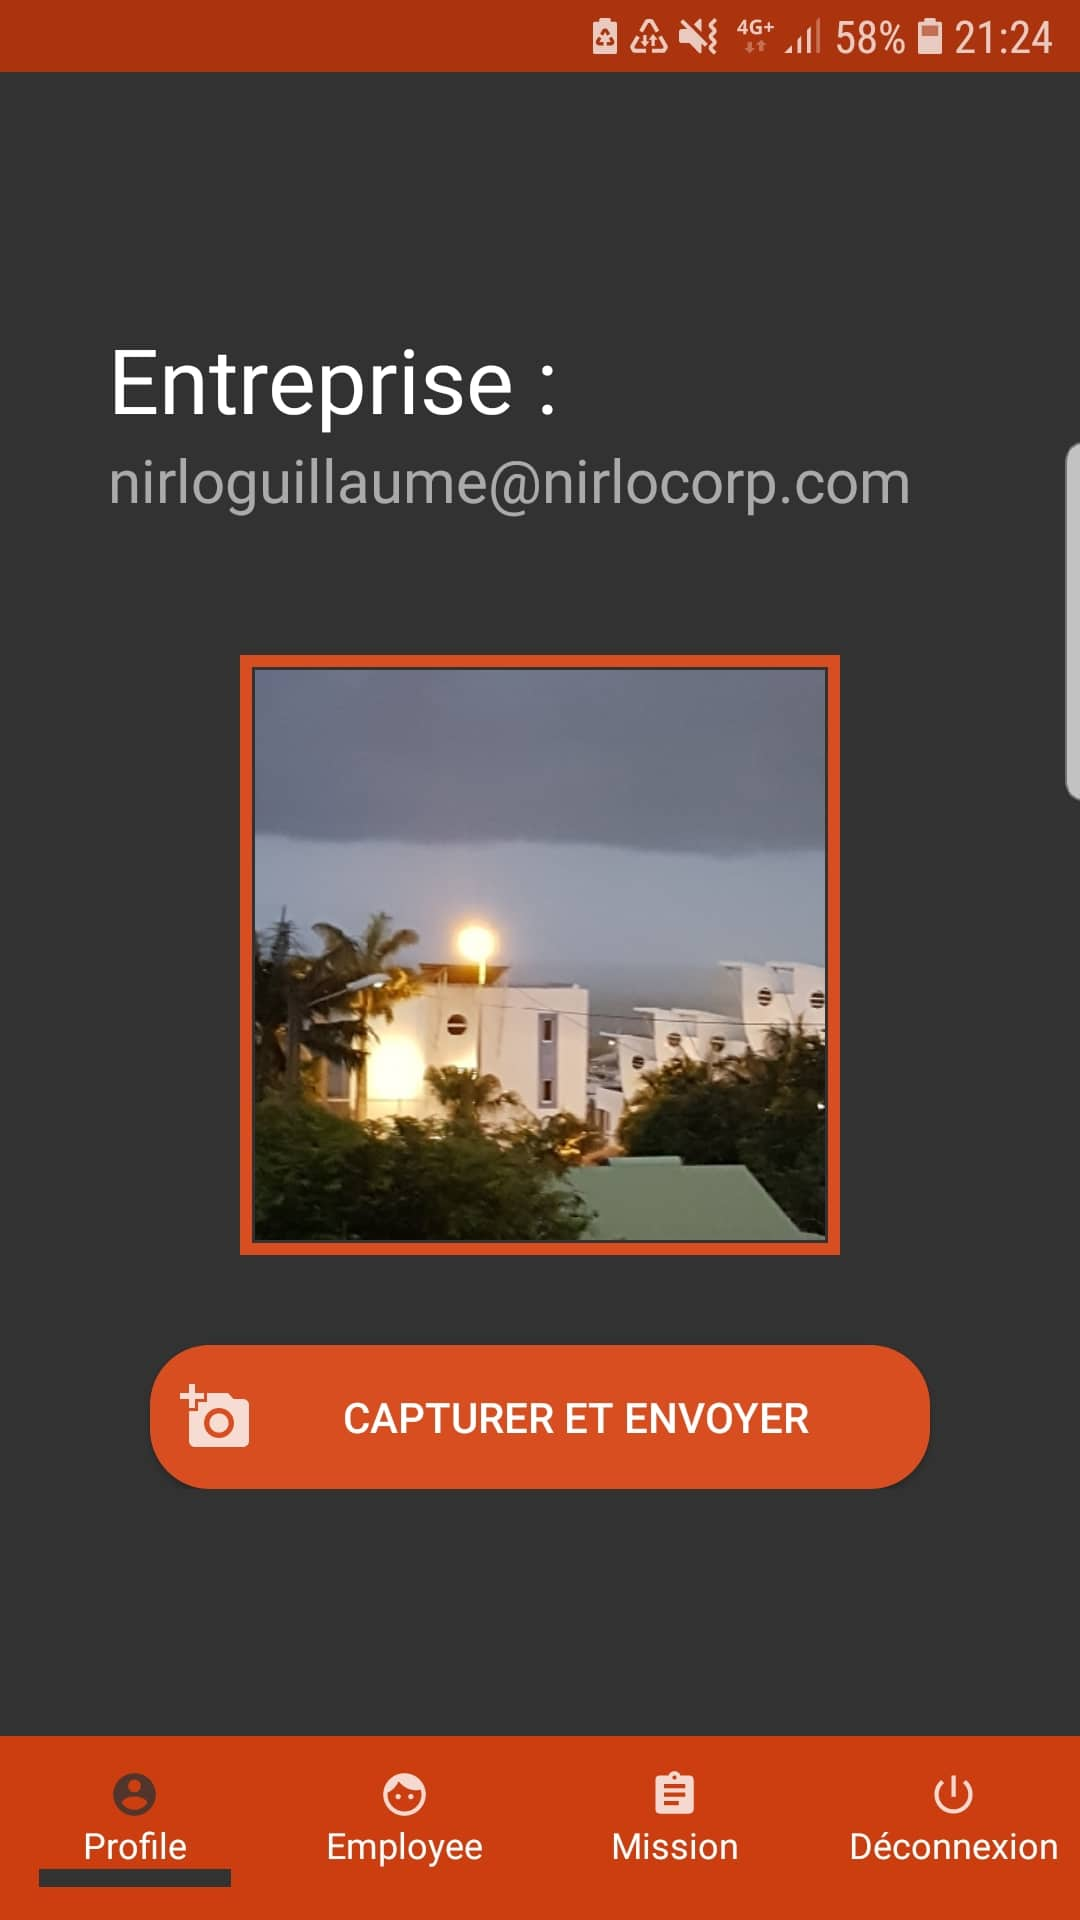
\includegraphics[scale=0.1]{profil.jpg}
    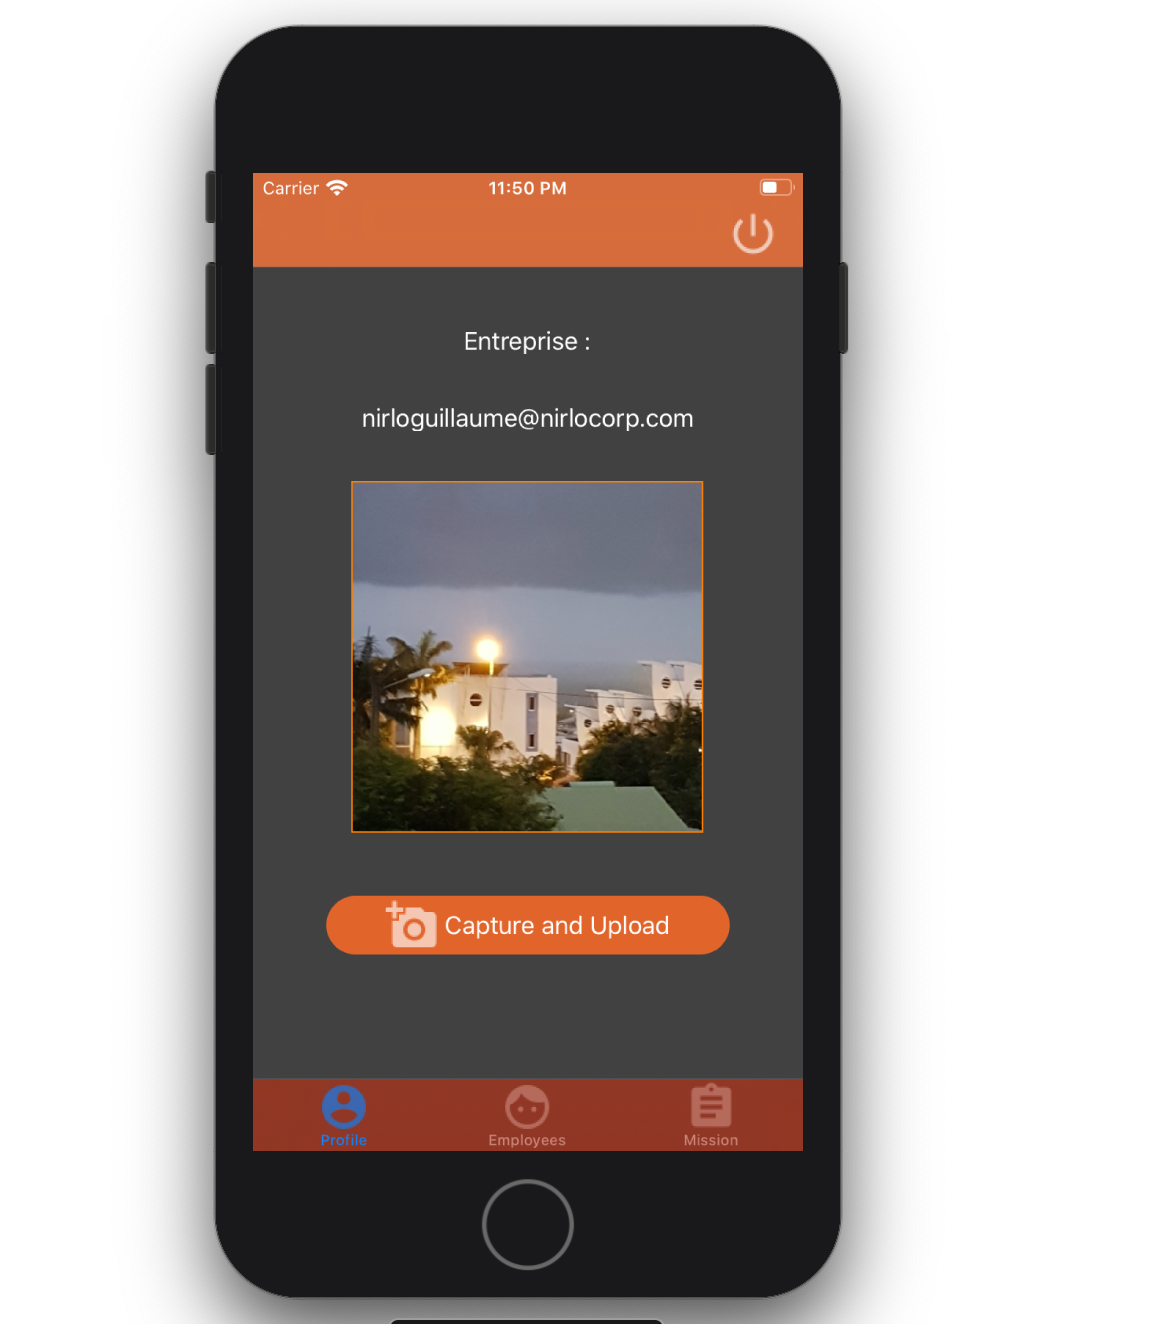
\includegraphics[scale=0.15]{profilIOS.png}
\end{center}

\newpage

\subsection{ Liste d'employés}

Dans l'onglet Employé, le gérant a juste accès à une liste en temps réel de tous les utilisateurs ayant un compte et il a la possibilité de supprimer un utilisateur en faisant glisser le cadre vers la droite ou la gauche Dans la version Android, il y aura par la suite une boîte de dialogue qui souvrira pour confirmer la suppression de cet utilisateur.

\begin{center}
	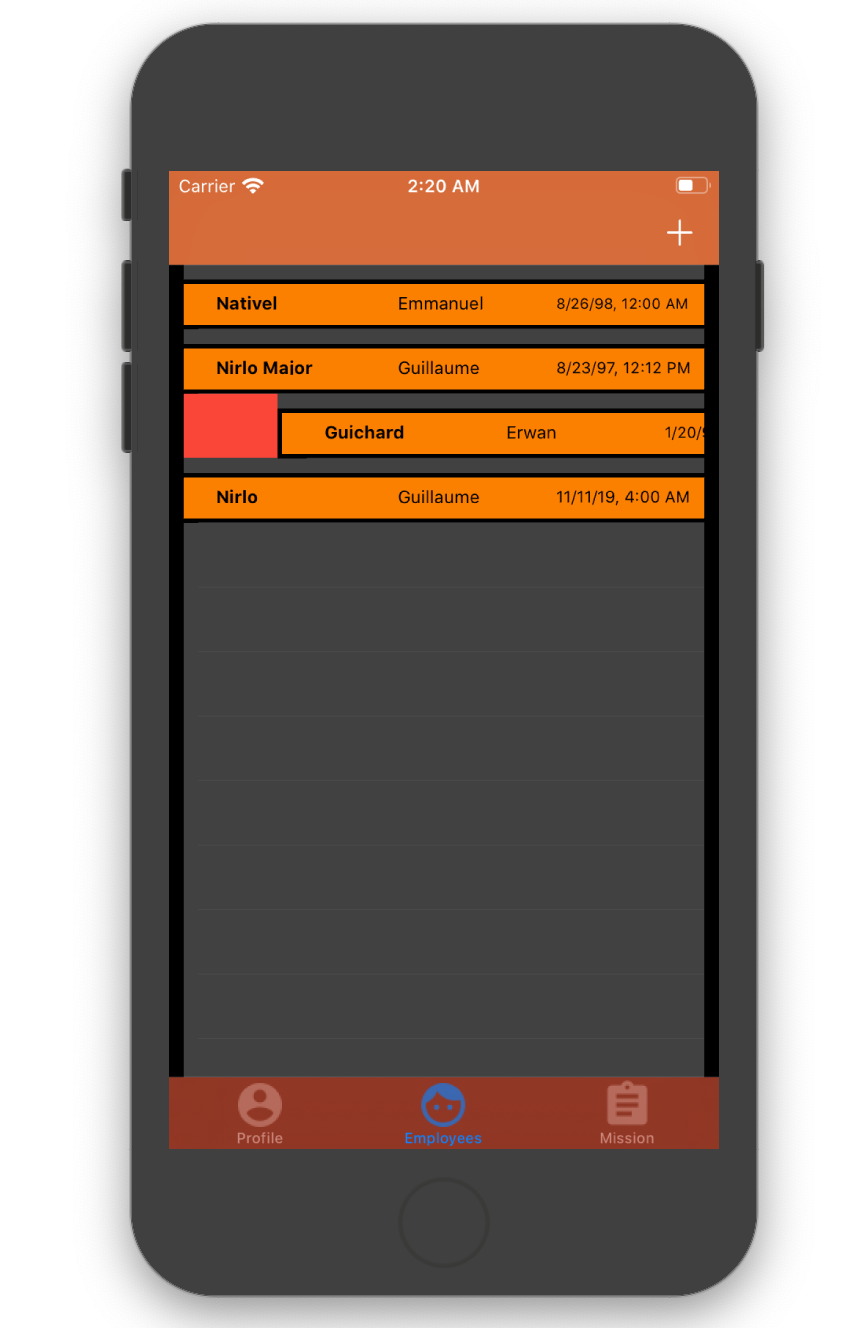
\includegraphics[scale=0.15]{listeEIOS.png}
    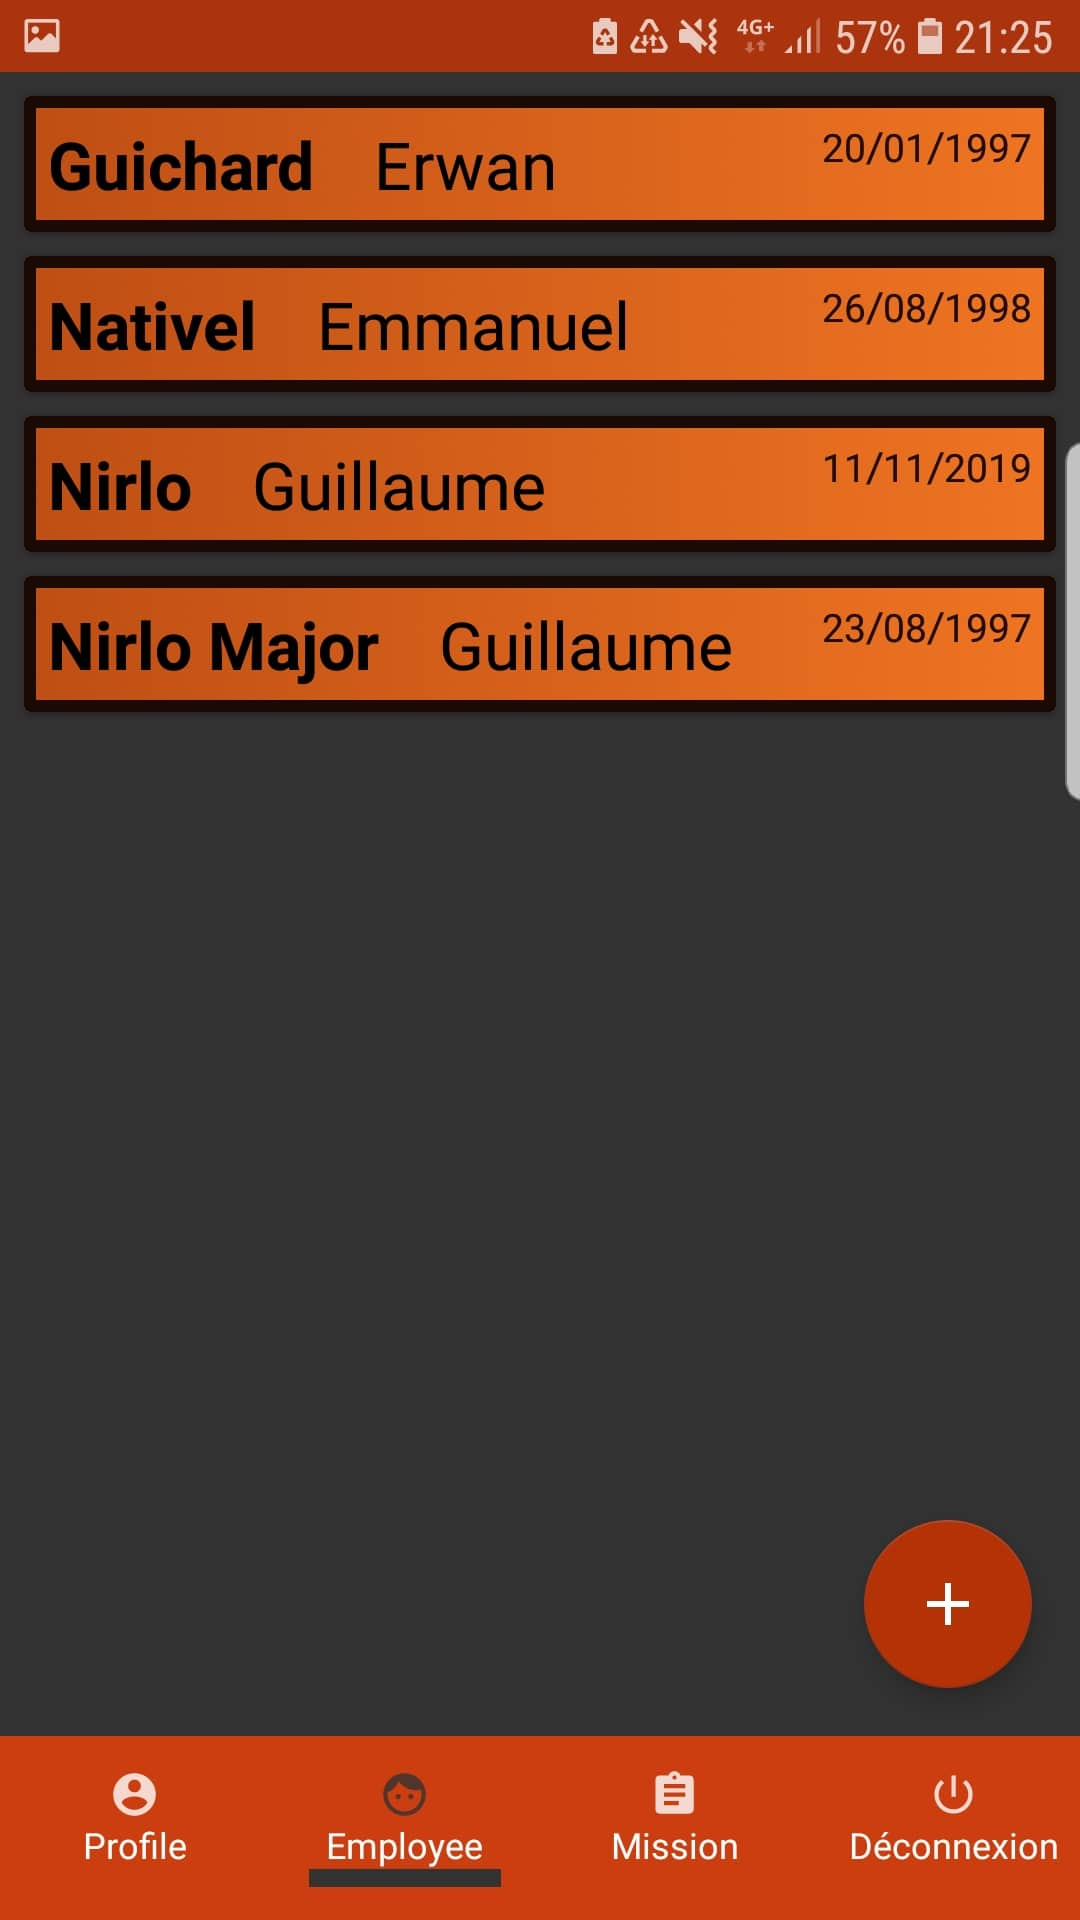
\includegraphics[scale=0.1]{listeE.jpg}
    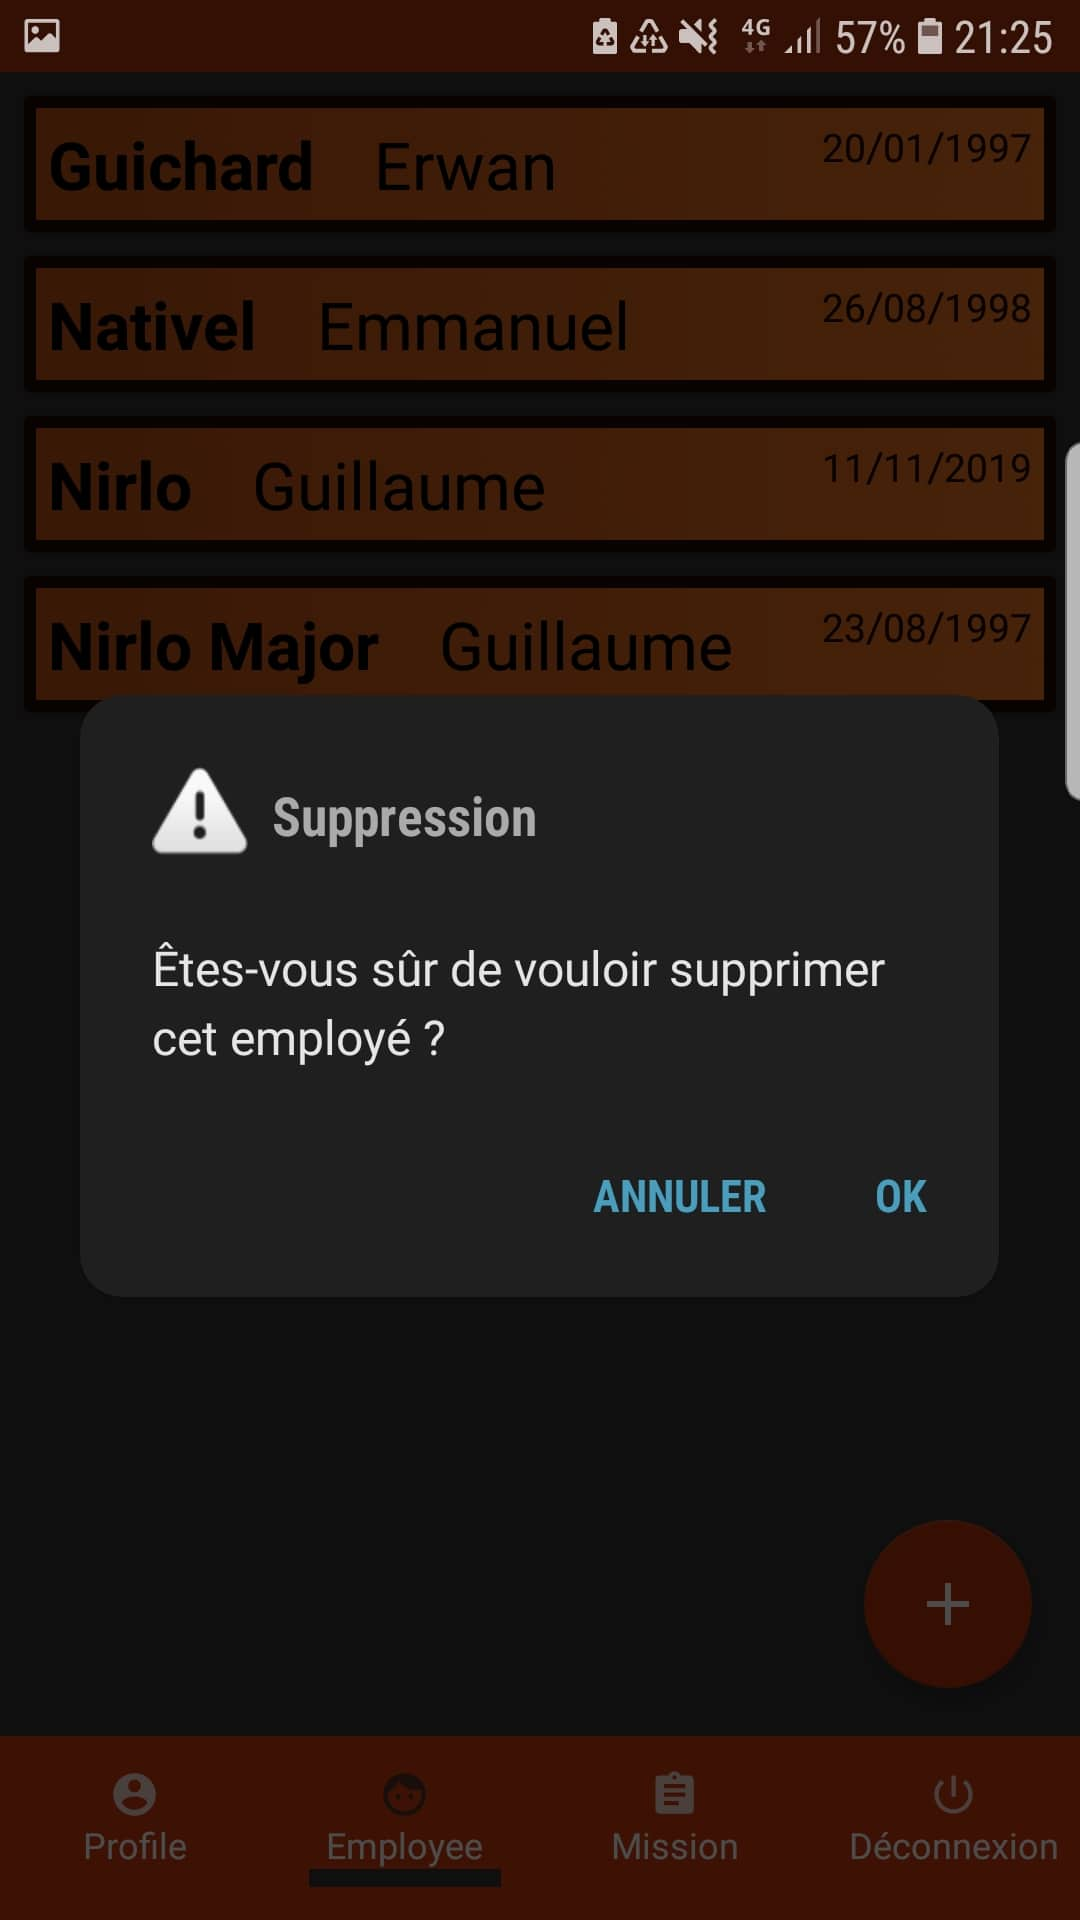
\includegraphics[scale=0.1]{suppE.jpg}
\end{center}

\subsection{Création d'un employé}

Dans ce même onglet, un bouton permet d'accéder à l'interface de création d'un nouvel employé. Le bouton calendrier permet d'ouvrir une petite interface qui permet de sélectionner la date facilement comme on peut le voir sur ces images :
\begin{center}
    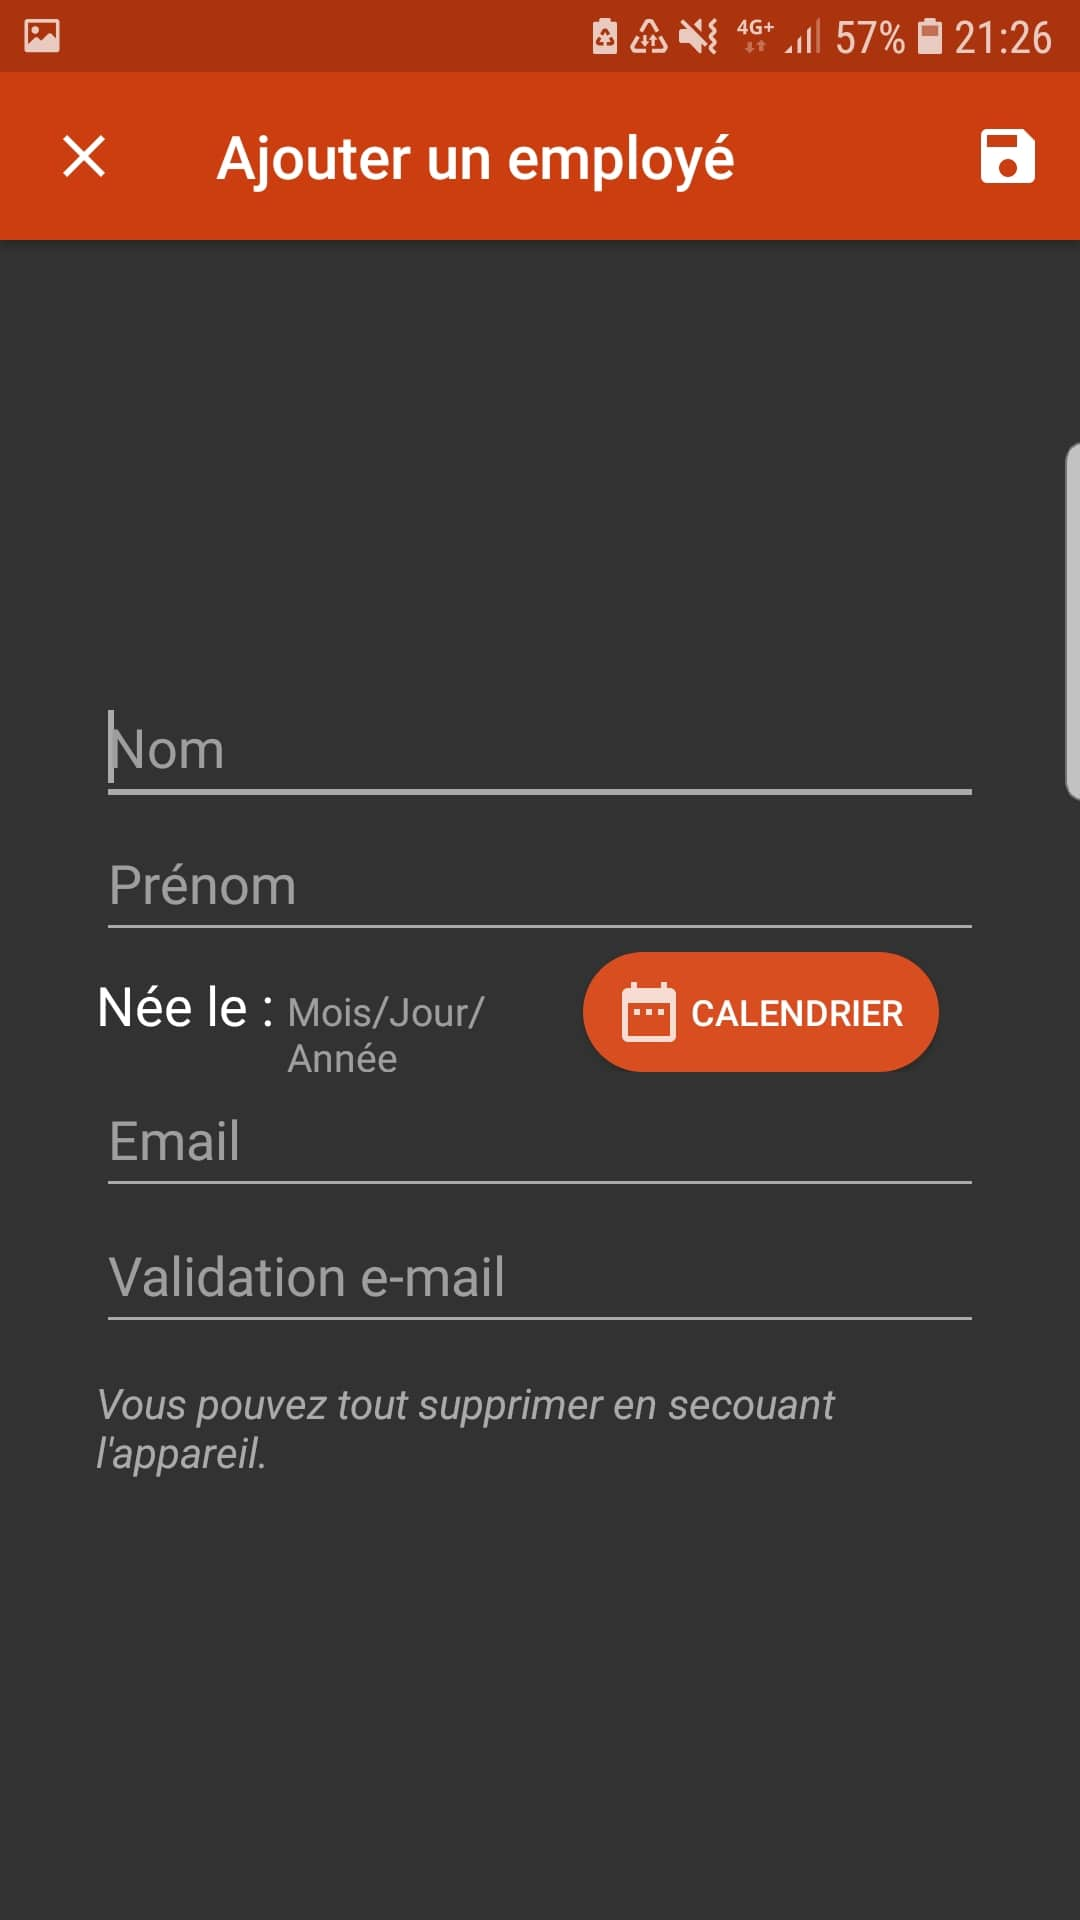
\includegraphics[scale=0.1]{ajoutE.jpg}
    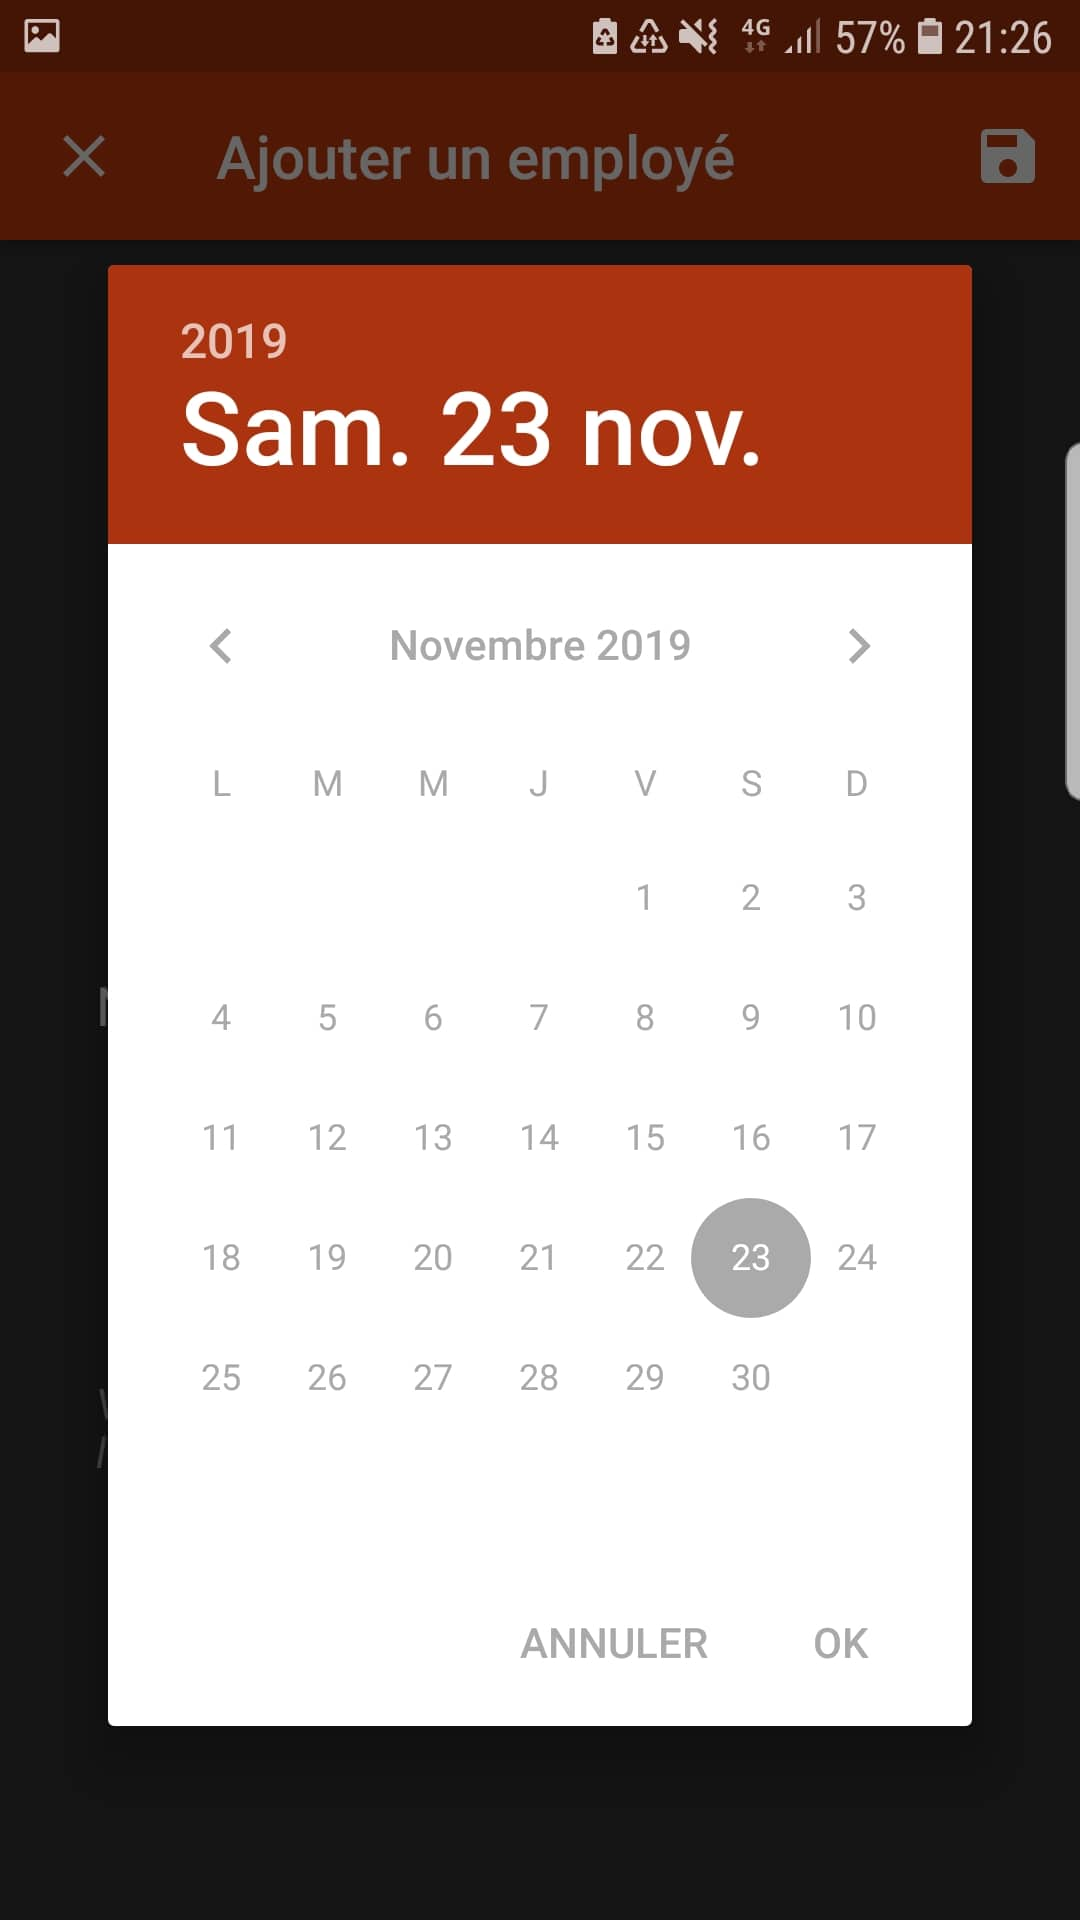
\includegraphics[scale=0.1]{calendar.jpg}
\end{center}

\newpage

La création d’un employé s’effectue en 2 parties. Il faut d'abord ajouter l’employé dans le module « Authentification » de Firebase, puis créer un document pour stocker les données de cet utilisateur dans la base de données. Le mot de passe lui est attribué aléatoirement.
Voici le code de création d'un employé sous iOS :
\begin{verbatim}
    let len = 8 //taille du mot de passe
    let pswdChars = "abcdefghijklmnopqrstuvwxyzABCDEFGHIJKLMNOPQRSTUVWXYZ1234567890"
    let rndPswd = String((0..<len).compactMap{ _ in pswdChars.randomElement() })
    if usernameTF.text != "" && emailTF.text != "" {
		us.createUser(withEmail: emailTF.text!, password: rndPswd) { (authResult, error) in
        if error != nil { print(error.debugDescription)}
        else {
            self.addUserDB(idU: self.us.currentUser!.uid)
            print("Inscription réussie")
            self.us.sendPasswordReset(withEmail: self.emailTF.text!) { (error) in
            if error != nil { print(error.debugDescription) }
            else { print("Send a password reset ")}
	}}}} 
\end{verbatim}

Si l'utilisateur souhaite vider rapidement le contenu des champs, il a la possibilité de secouer le téléphone afin d'ouvrir une boite de dialogue pour confirmer la suppression des zones de textes.

Pour valider la création de l'utilisateur le gérant devra cliquer sur la disquette en haut à droite dans la barre du menu. 
Une fois la création de l'employé validée, Firebase va lui envoyer un mail contenant un lien pour réinitialiser son mot de passe.  Voici un exemple du mail que recevra chaque nouvel employé avant leur première connexion :
\begin{center}
    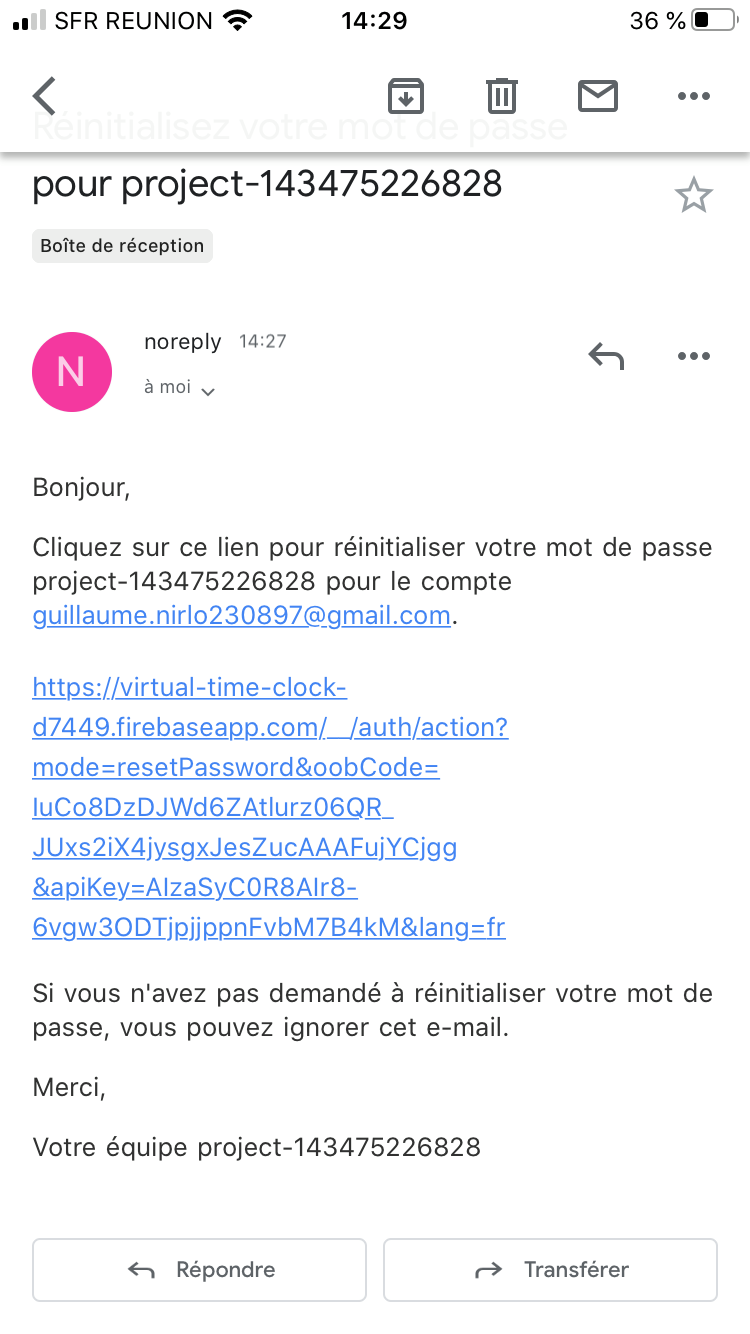
\includegraphics[scale=0.15]{mail.png}
\end{center}

\newpage

\subsection{Liste des missions}

Le gérant possède une vue sur l’ensemble des missions lui permettant d’ajouter ou de supprimer les missions actuelles. Chaque cellule est composée d’un bref affichage permettant de distinguer rapidement les différents enjeux.

\begin{center}
    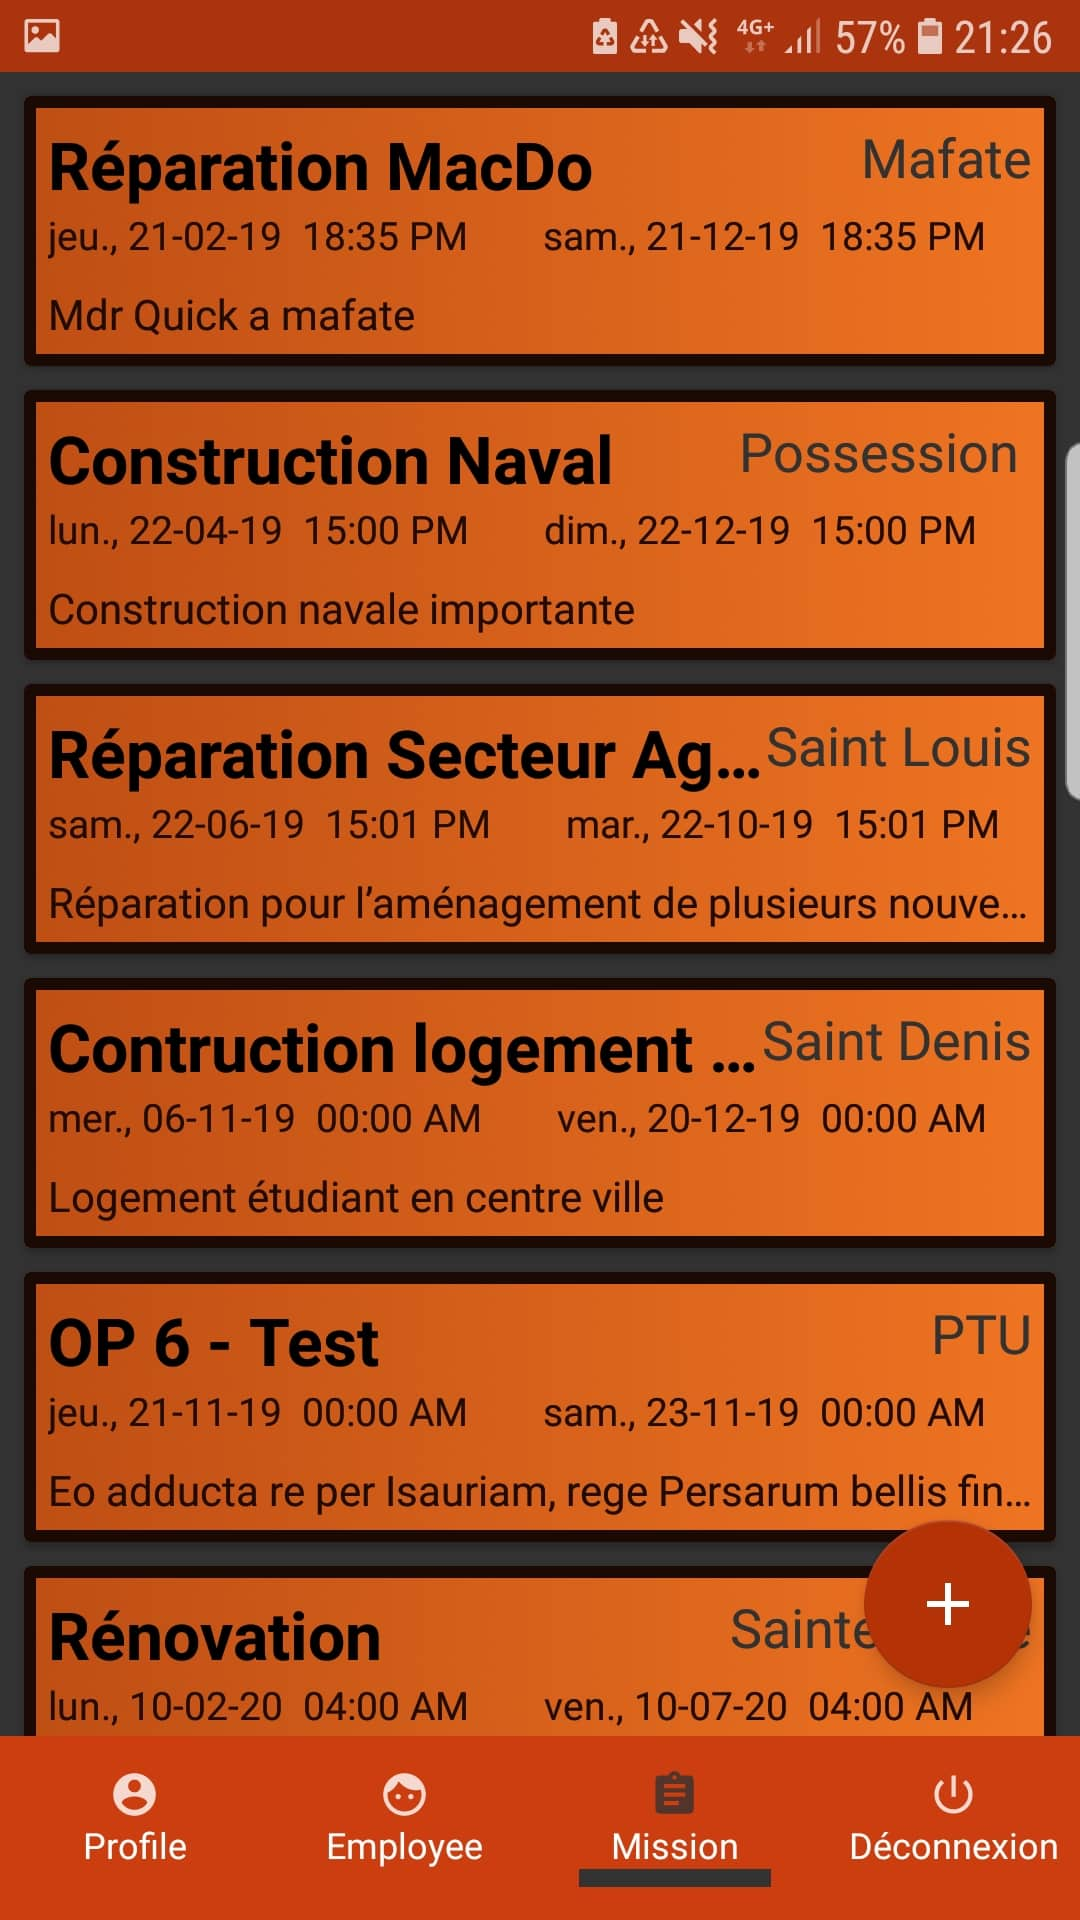
\includegraphics[scale=0.1]{listeM.jpg}
    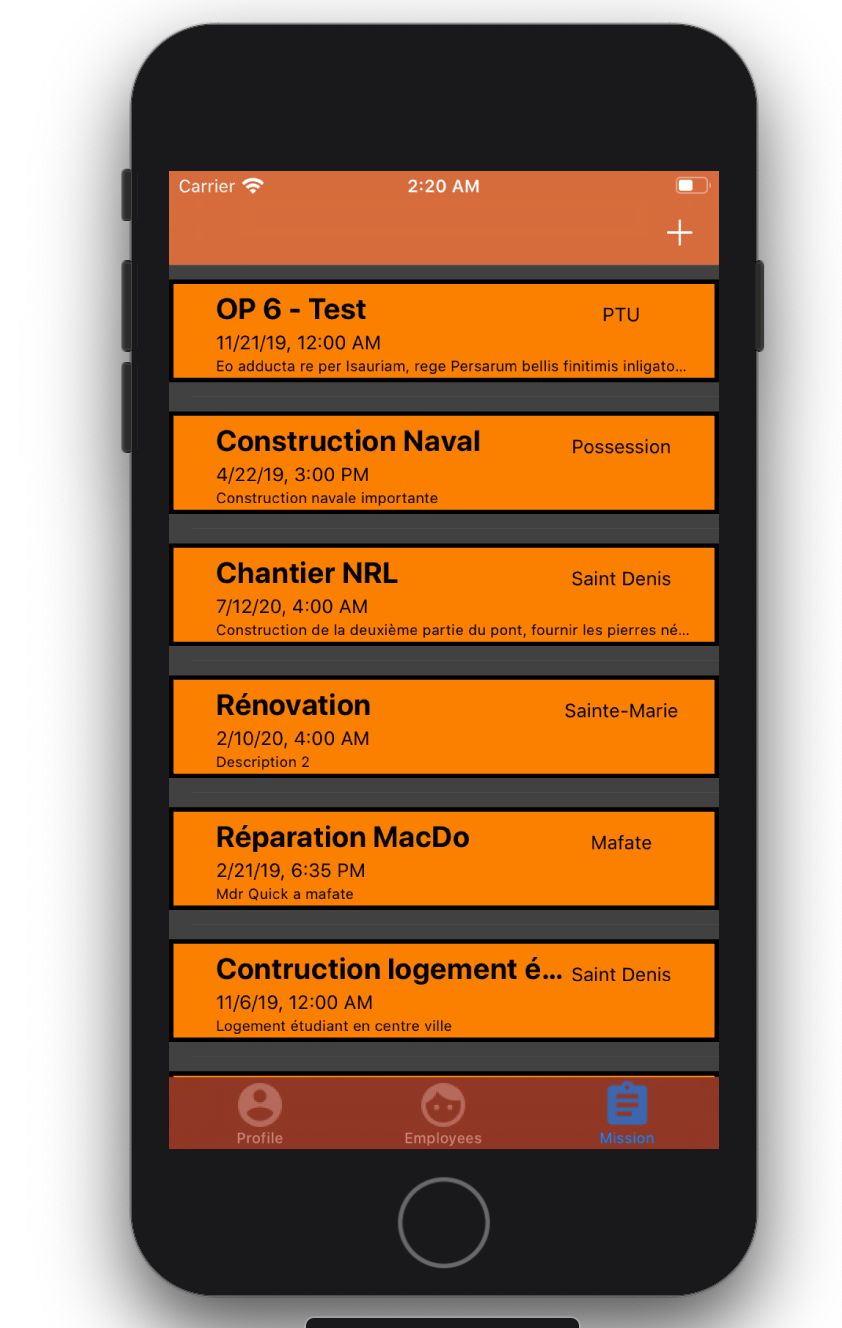
\includegraphics[scale=0.15]{listeMIOS.png}
\end{center}

\subsection{Création de mission}

\begin{center}
    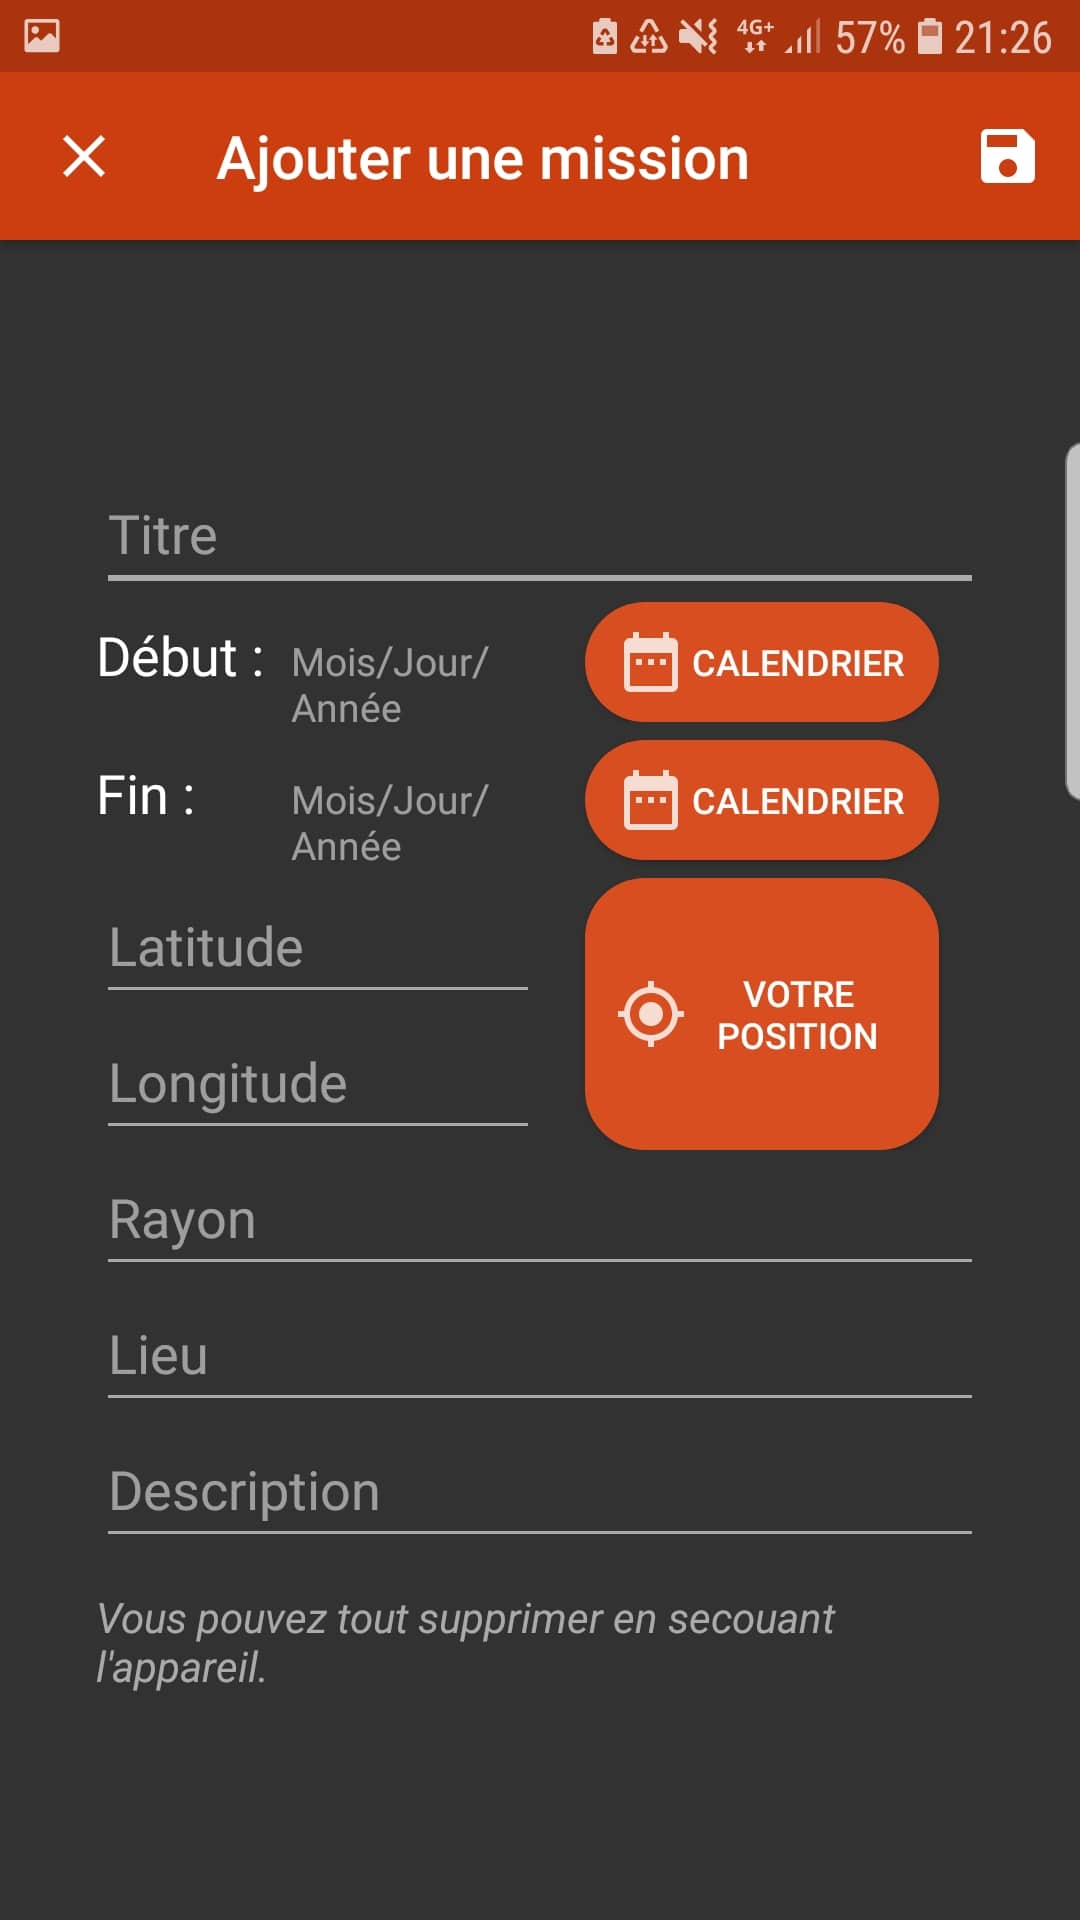
\includegraphics[scale=0.1]{ajoutM.jpg}
    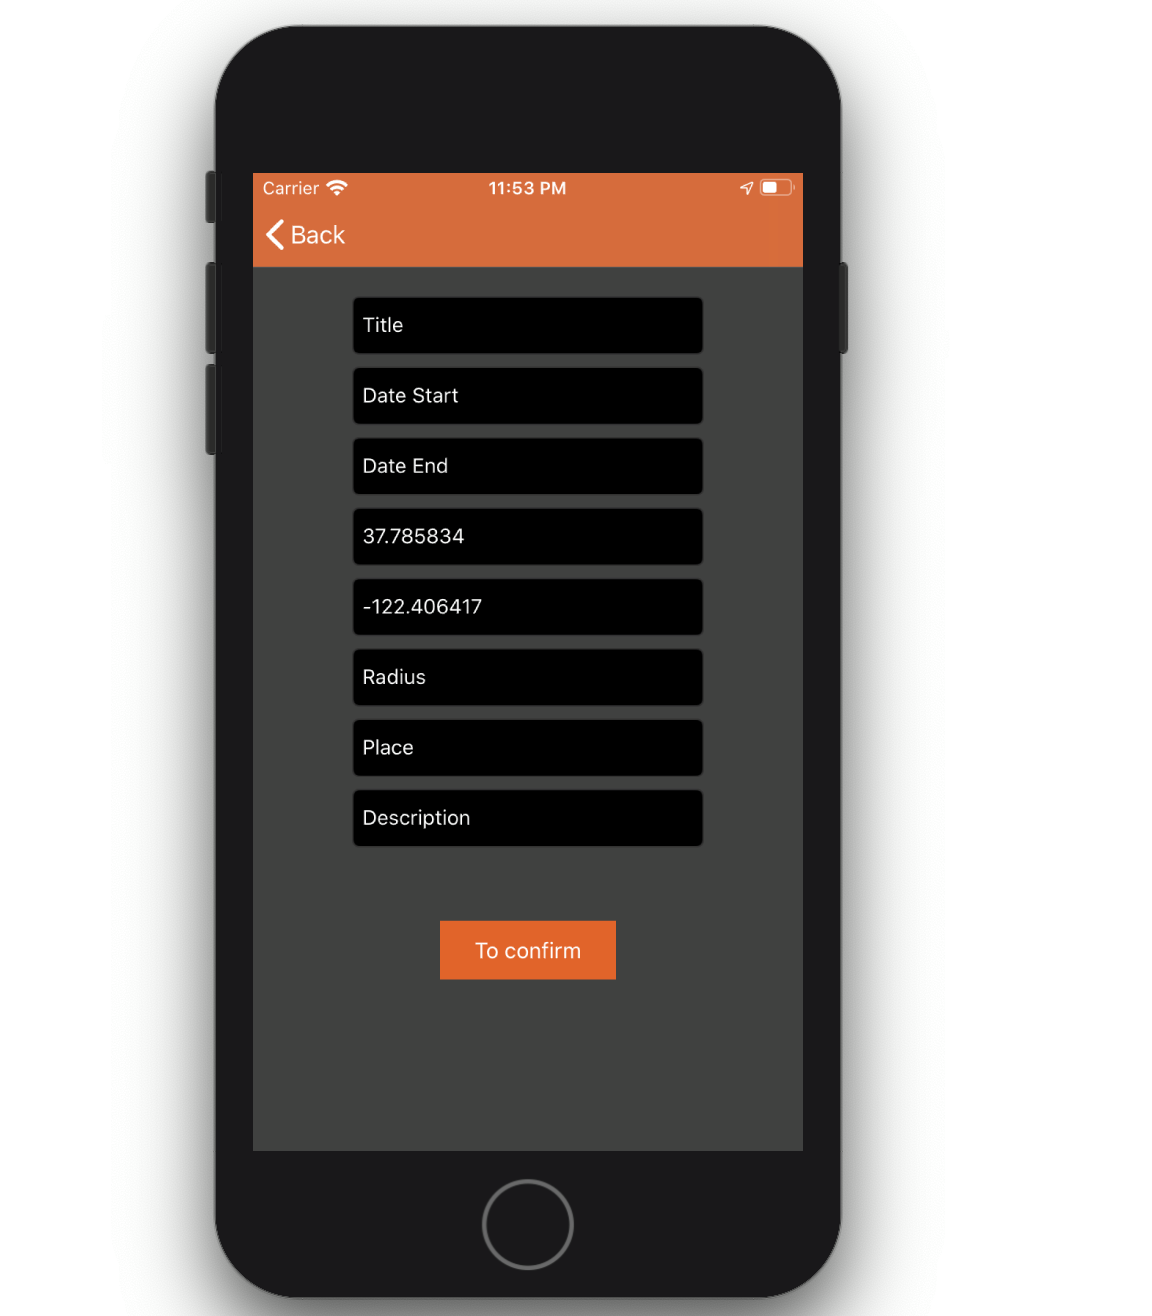
\includegraphics[scale=0.15]{ajoutMIOS.png}
\end{center}
L'onglet Mission contient aussi un bouton flottant pour accéder à l'interface de création de mission. Dans la version Android, la localisation de la zone de la mission peut être saisie manuellement ou être récupérée automatiquement en cliquant sur le bouton localisation. Dans la version iOS, dès l'affichage du formulaire, l'application demande l’autorisation de récupérer les coordonnées actuelles afin de remplir automatiquement les champs.
Pour sauvergarder il faut que toutes les données soient saisis et que la date de départ soit plus petites que la date de fin.Voici un exemple d’écriture dans la base, il faut avant tout ouvrir la collection que l’on veut éditer puis écrire tous les champs manuellement et convertir les type du langage en types firebase si nécessaire.

\newpage

\begin{verbatim}
    let db = Firestore.firestore()
        let userDoc = db.collection("missions")
        let dateCourante: Timestamp = Timestamp(date: datePicker!.date);
        let dateCourante2: Timestamp = Timestamp(date: datePicker2!.date);
        let getrayon: String = ""+rayonTF.text!
        let rayonConvertDouble = Double(getrayon)
        let rayonFinal: Double = Double(rayonConvertDouble!)
        let pos: GeoPoint = GeoPoint(latitude: latitude, longitude: longitude )
        
        userDoc.document().setData([
            "debut": dateCourante,
            "description": descTF.text!,
            "fin": dateCourante2,
            "lieu": lieuTF.text ?? "",
            "localisation": pos,
            "rayon": rayonFinal,
            "titre": titleTF.text ?? "",
        ])
\end{verbatim}

\subsection{Détail d'une mission}

Dans l'onglet Mission, le gérant a la possibilité de consulter les détails de chaque mission en cliquant dessus. Si la description est trop longue le gérant à la possibilité de scroll.
\begin{center}
    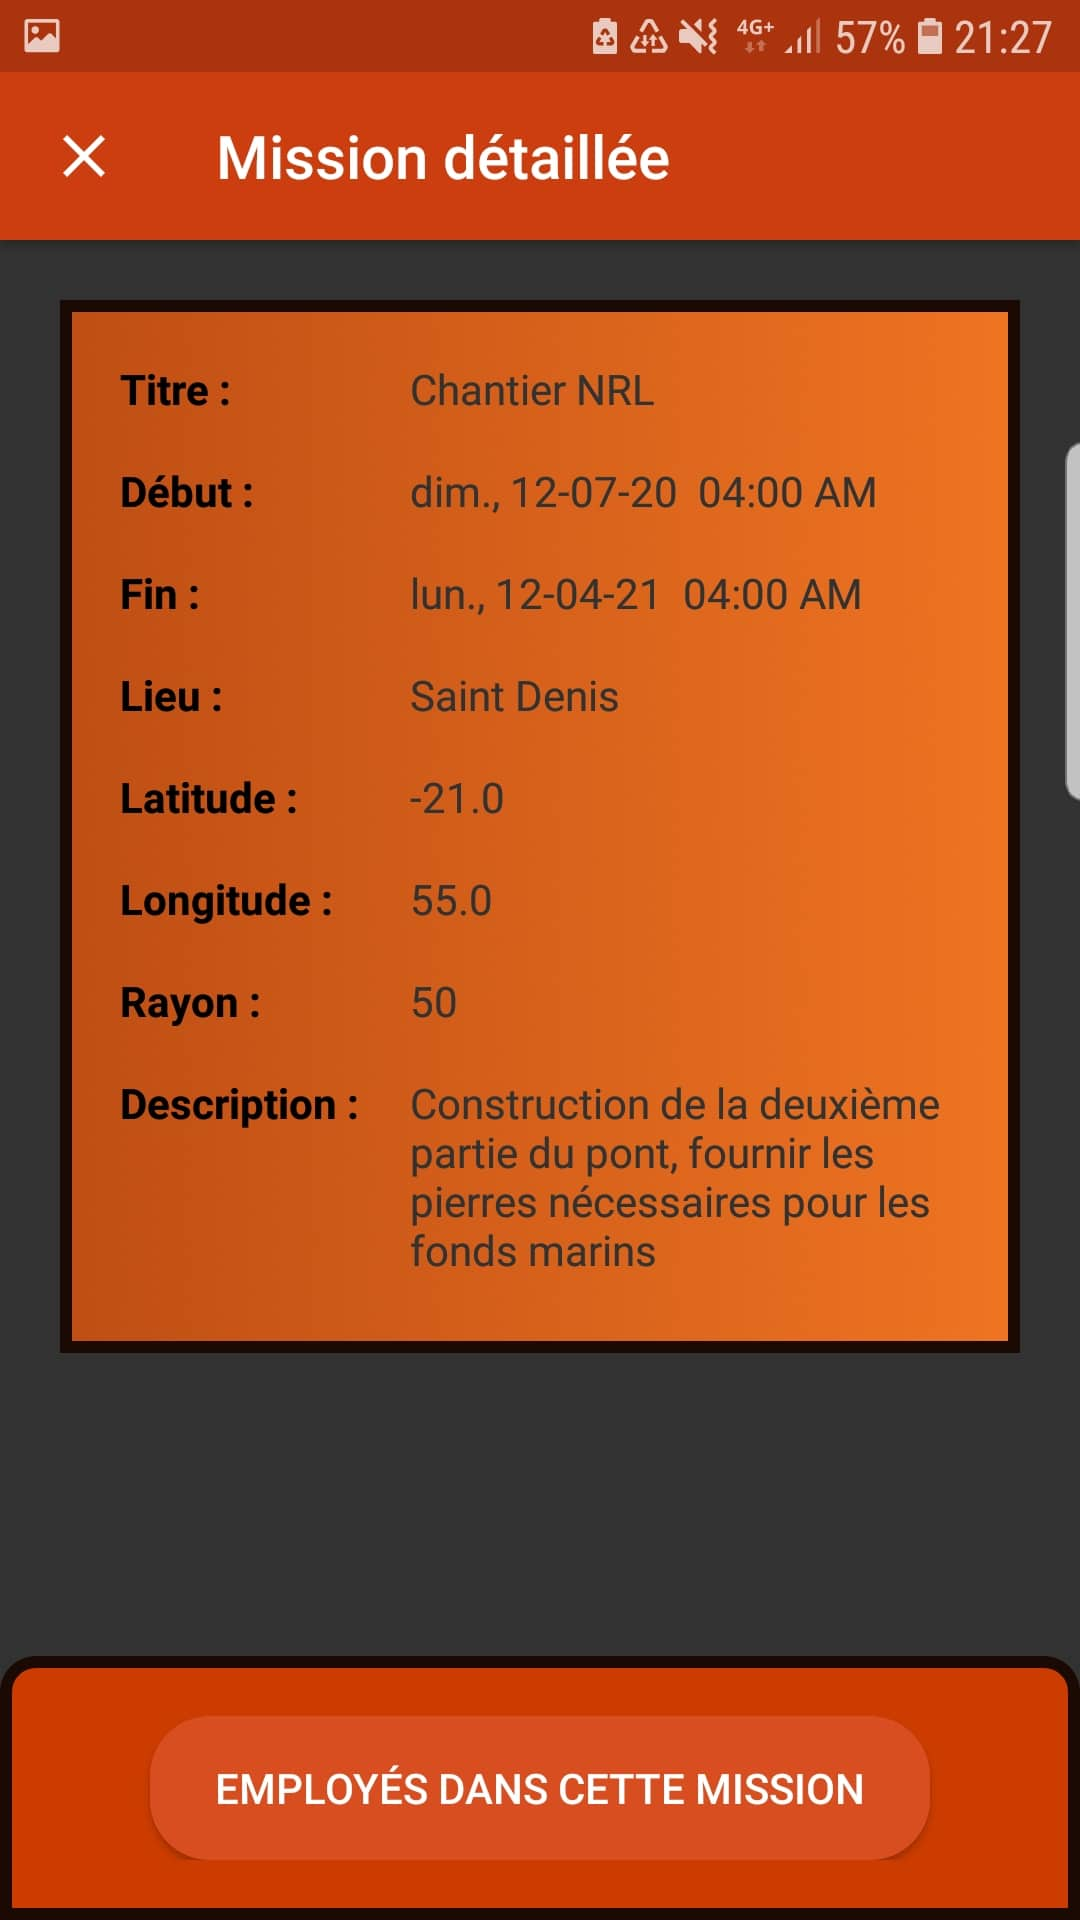
\includegraphics[scale=0.1]{detailM.jpg}
    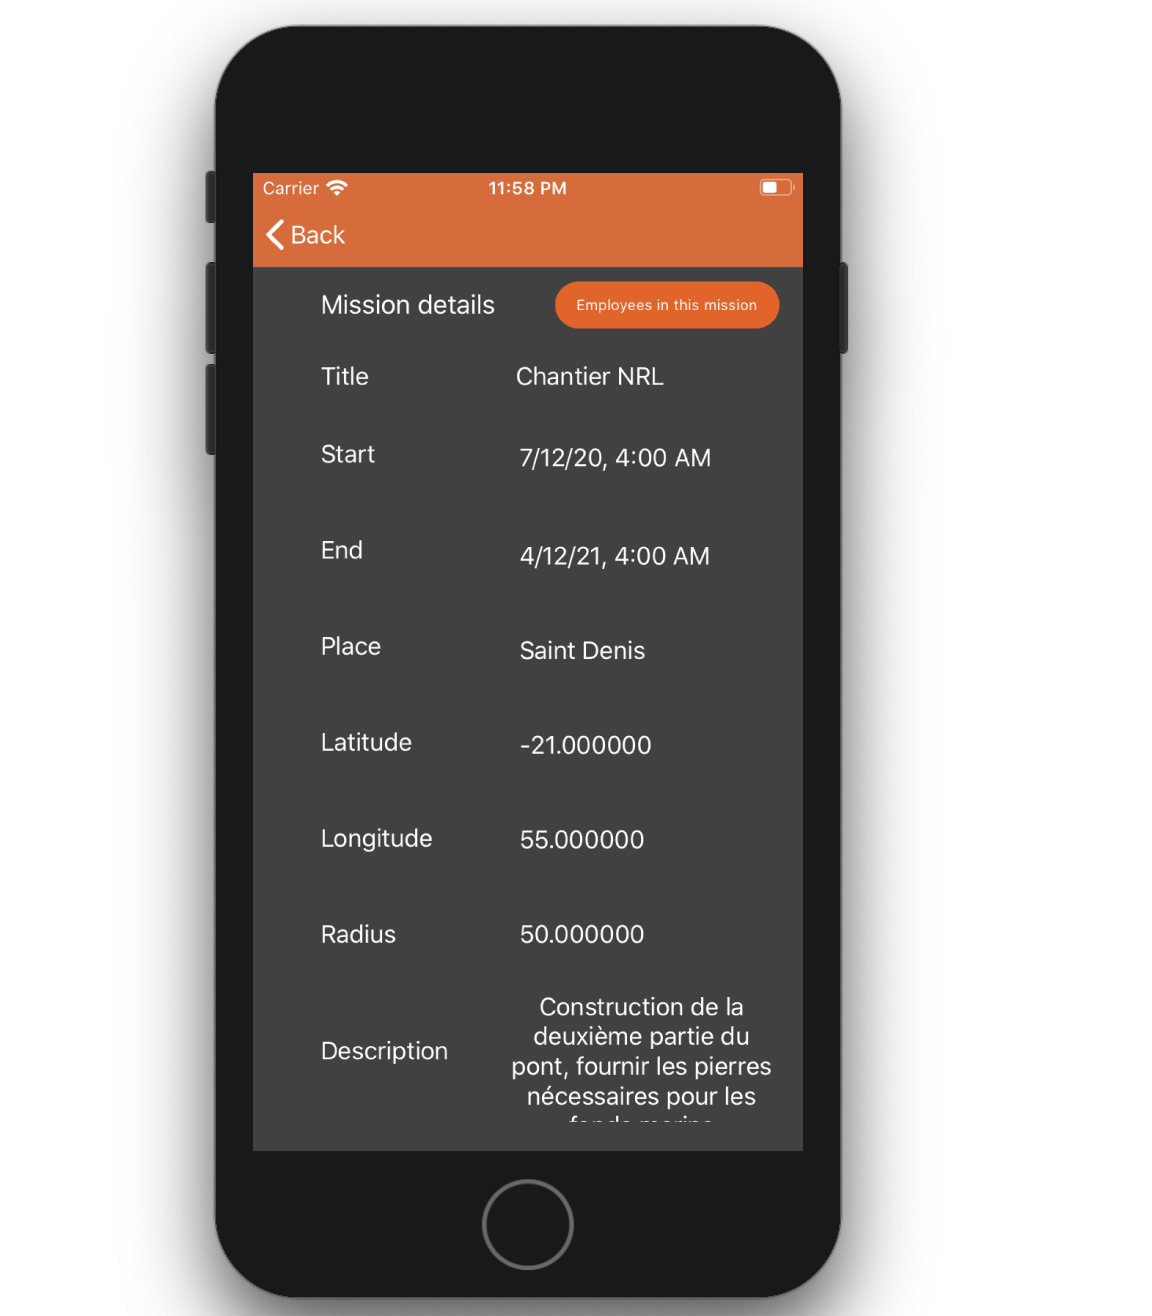
\includegraphics[scale=0.15]{detailMIOS.png}
\end{center}

\newpage

\subsection{Consultation de la présence des employé }

Dans la vue de détail des missions, le gérant peut accéder à la liste des employés présents acutellment sur les lieux de la missions en cliquant sur le bouton "Employés dans cette mission". Pour chacun des employés ayant pointé sur cette missions, le gérant peut voir son nom, prénom, la date de dernière mise à jour et si il est présent ou absent des lieux de la mission en temps réel. Si l'employé est sur les lieux, l'image d'un pointeur vert s'affiche, sinon c'est un pointeur rouge barré qui est affiché. Les données peuvent petre actualisées en appuyant sur le bouton "Update".
\begin{center}
    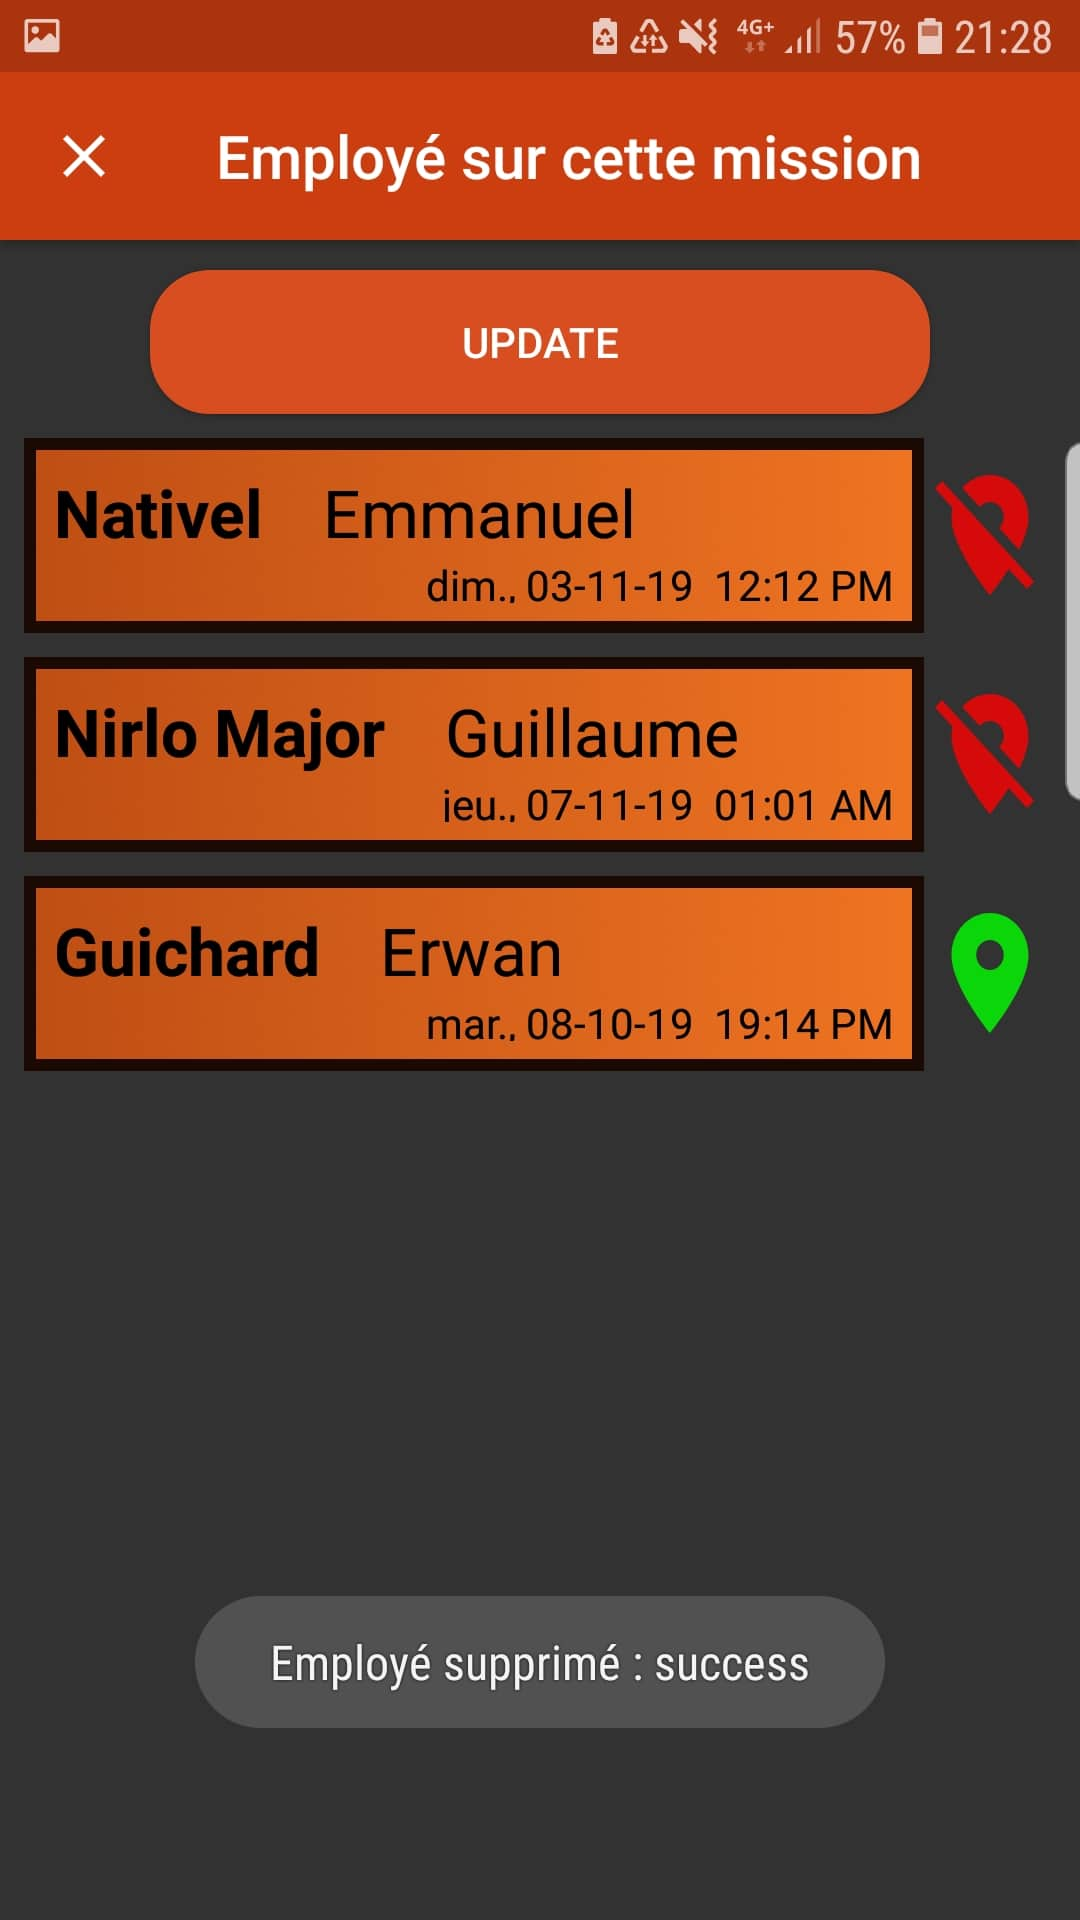
\includegraphics[scale=0.1]{pointage.jpg}
    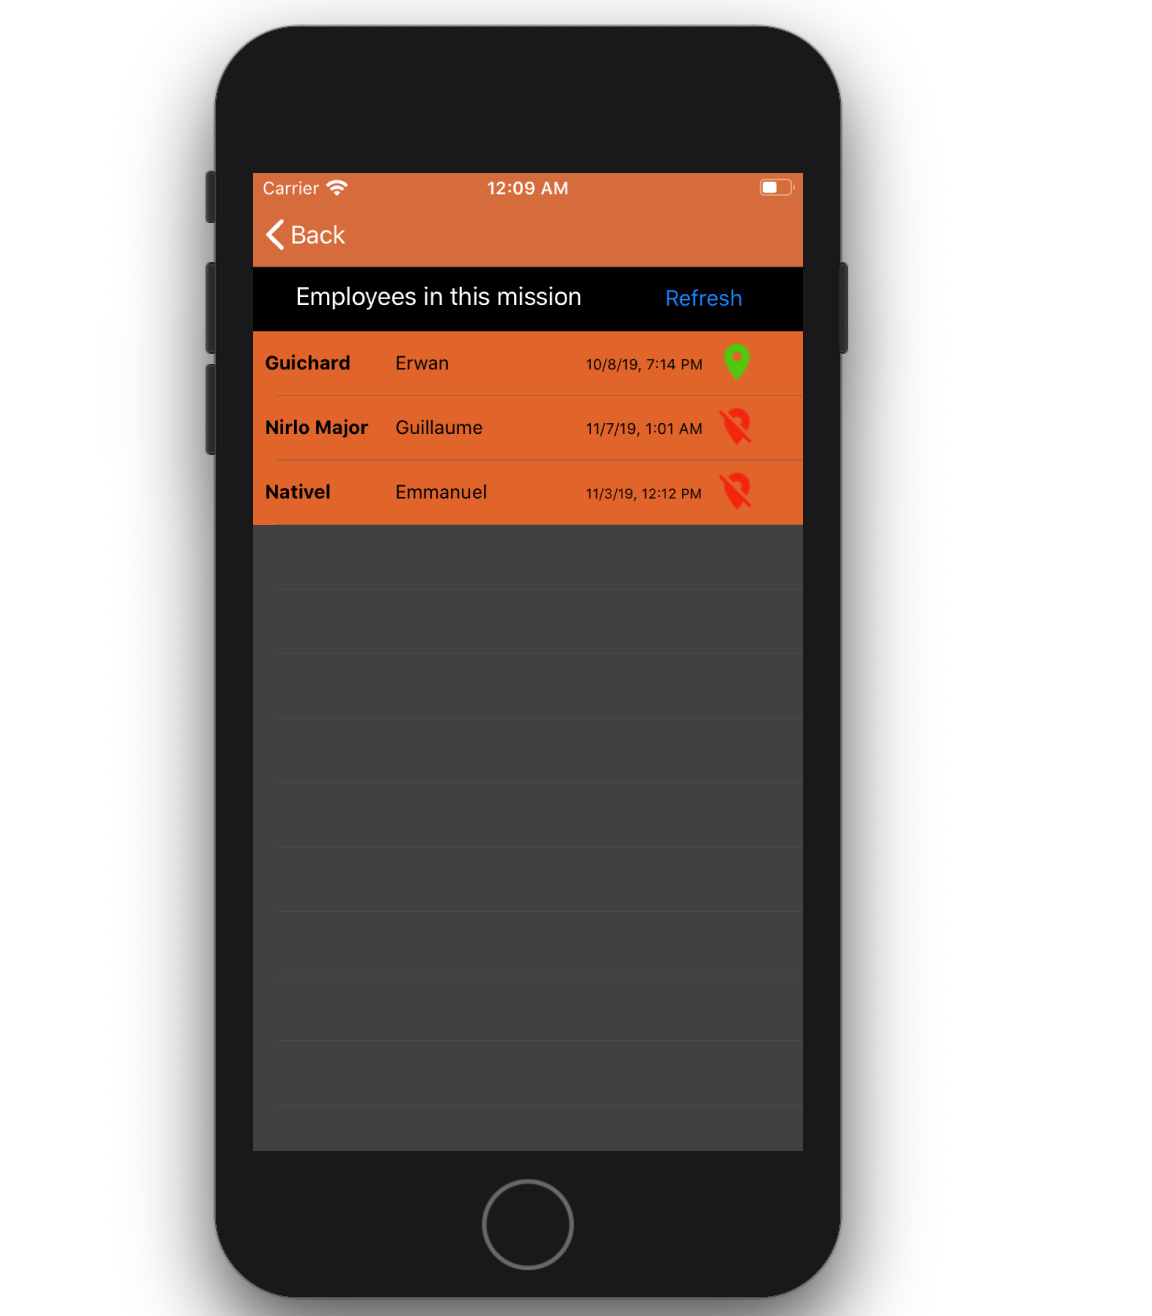
\includegraphics[scale=0.15]{pointageIOS.png}
\end{center}

Cette partie a été une des plus difficile à réaliser à cause de la gestion des requêtes asynchrones. En effet, nous avons du lire dans deux collections différentes en même, tout en synchronisant les lectures dans les deux collections et l'affichage des données. 
Tout d'abord, nous avond du récupérer l'id de la mission choisie par le gérant par le biais de la fonction prepare sous iOS : 

\begin{verbatim}
override func prepare(for segue: UIStoryboardSegue, sender: Any?) {
        if segue.identifier == "goToPointEmp" {
            let destination = segue.destination as! ListPointEmpController
            destination.missionID = mission!.id
} }
\end{verbatim}

Puis, il a fallut lire dans la collection "pointage" afin de récupérer le document associé à cette mission, grâce à son id. A partir de là, nous avions accès à la liste des id des employés qui ont pointés sur cette mission, la date de la dernière information de pointage et si l'employé a été présent ou non à cette date. Cependant, arrivé à ce niveau, il nous manquait encore le nom et le prénom de cet employé. Pour cela, nous avons du lire dans la collection "utilisateurs", pour chacun des id récupérés auparavent. 
Voici le code iOS correspondant : 

\newpage

\begin{verbatim}
db.collection("pointage").document(missionID).collection("pointageMission")
.getDocuments() { (query, err) in
if let err = err {print("Erreur : Impossible d'obtenir les missions ! \(err)")}
else {
  print("Document récupéré !")
  for document in query!.documents {
    let userID = document.documentID
    let estPresent = document.get("estPresent") as! Bool
    let dateTimestamp = document.get("date") as! Timestamp
    let date = dateTimestamp.dateValue()
    var name: String = ""
    var firstname: String = ""
    if userID != "" {
      self.db.collection("utilisateurs").document(userID).getDocument { (document2, error) in
      if let error = error {
      print("Erreur : Impossible d'obtenir les utilisateurs ! \(error)")
      } else if let document2 = document2, document2.exists {
      firstname = document2.get("prenom") as! String
      name = document2.get("nom") as! String

      print("\(name)name")
      print("\(firstname)firstname")
      self.pointEmp.append(PointEmp(id: userID, nom: name, 
      prenom: firstname, date: date, estPresent: estPresent))
      self.tableView.reloadData() // Rechargmement des données des cellules
    } else {
		print("L'utilisateur n'existe pas")
        self.db.collection("pointage").document(self.missionID).collection("pointageMission")
        .document(userID).delete()
}}}}}}
\end{verbatim}

\subsection{Déconnexion}

Le bouton Déconnexion ouvre simplement une boîte de dialogue qui demande au gérant si il souhaite vraiment être déconnecté et si il valide il sera ramené sur l'interface de connexion ou il devra se réauthentifier.
\begin{center}
    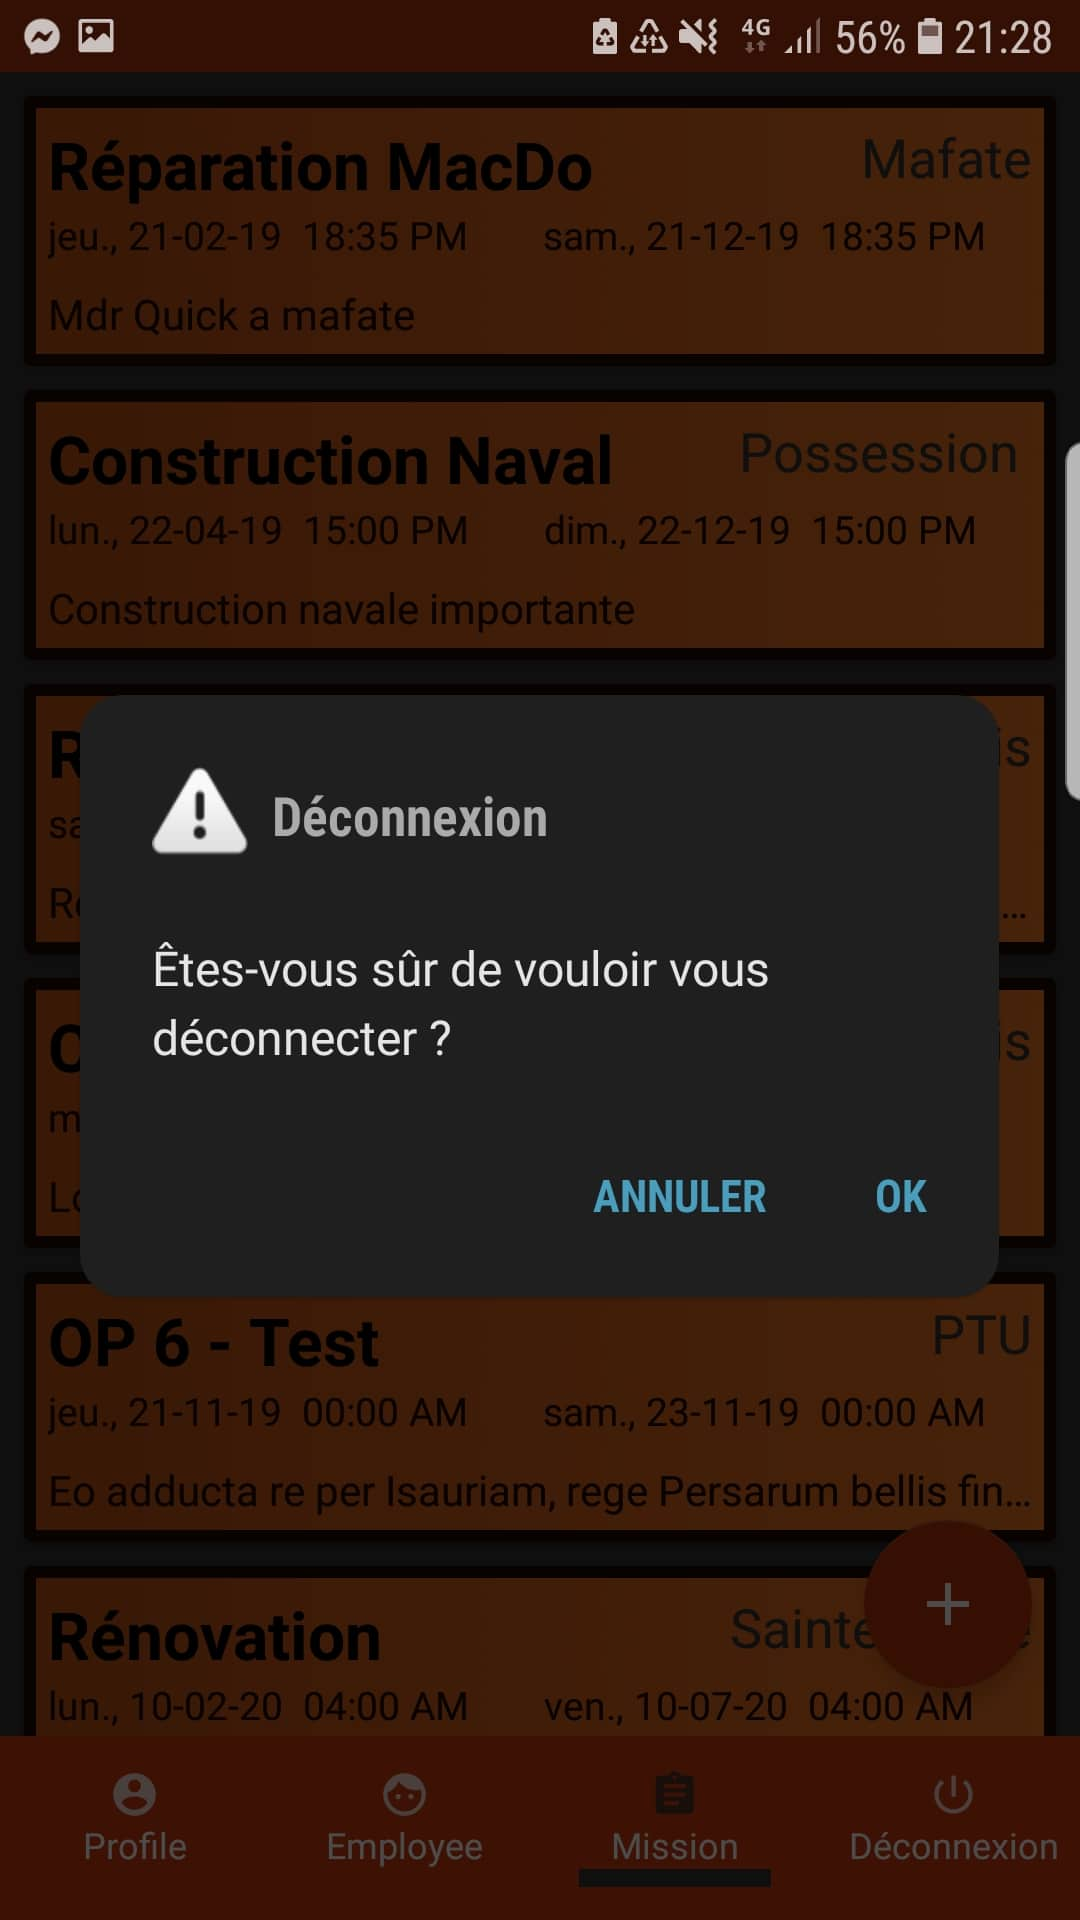
\includegraphics[scale=0.1]{deco.jpg}
\end{center}

\newpage

\section{Limites rencontrées}

Nous avons rencontré plusieurs limites pendant le développement de l'application. 
Premièrement, par manque de temps, il n'est pas possible de modifier des missions ou des employés, seules les fonctionnalités d'ajout et de supression ont été implémentées. 
De plus, nous n'avons pas eu le temps de gérer l'affichage de la présence des employé en temps réel. Pour combler cela, nous avons ajouté un bouton d'actualisation. 
La création d’employés a aussi été délicate. En effet, après avoir créer un employé, ce dernier se connectait automatiquement en écrasant l’ancienne session connectée, ce qui pouvait causer des problèmes notamment à cause du fait qu’un client ne peut se connecter sur l'application d’un gérant.

\section{Difficultés rencontrées }

La principale difficulté que nous avons rencontré a été l'utilisation de Firebase, car aucun d'entre nous n'avait utilisé cette plateforme auparavant. Notamment pour gérer les requêtes asynchrones de firebase. En effet, il arrivait que les données étaient chargées après l'affichage de la vue. 
Au niveau de l'application des employés, la partie la plus difficile a été la gestion des alertes de proximité. Ce problème a été réglé grâce au singleton design pattern.

\section{Conclusion}

Pour conclure, nous avons réussi à réaliser l'objectif principal qui était de faire communiquer les deux applications afin de contrôler l'assiduité des employés au travail. 
De plus, nous avons découvert la plateforme Firebase qui s'avère très utile lorsque l'on veut se concentrer uniquement sur le front de notre application. 
Certaines fonctionnalités n'ont pas pu être implémentées et pourraient faire l'objet de futures évolutions. 


%%% La bibliographie:
\bibliographystyle{plain}
\bibliography{ma_biblio}

\end{document}
